\chapter{Experiments}
\label{sec:experiments}
We ran several experiments to evaluate the performance characteristics of the implemented algorithm, compare its performance on the \ac{wse} to highly optimized implementations on traditional \ac{hpc} architectures (\ac{cpu}, \ac{gpu}), and assess the possibility of further optimizing our implementations.

\section{Methodology}
All experiments for the Cerebras \ac{wse} were conducted using the cycle-accurate simulator provided in the Cerebras SDK (v1.3.0).
Due to the significant computational resources required, simulations were limited to a smaller number of \acp{pe} (up to 50x50) and iterations than would be used on physical hardware.
To estimate the performance our implementation could achieve on a full system, we extrapolated our results to larger numbers of \acp{pe} and iterations.
We extrapolate to more \acp{pe} by assuming perfect weak scaling, meaning that the cycle count doesn't increase if more \acp{pe} are used when keeping the workload per \ac{pe} constant.
This assumption is supported by two key pieces of evidence: The results from \citeauthor{jacquelin2022scalable} \cite{jacquelin2022scalable} who achieve near-perfect weak scaling for their implementation of a 3D stencil on a \ac{wse}-2 system.
Furthermore, we run our own weak scaling experiments on the simulator and find that the cycle count is almost constant when increasing the number of \acp{pe} (\autoref{sec:weak_scaling}).

We measure the runtime of our implementations by calculating it from the recorded number of clock cycles used per iteration and the clock speed of the \ac{wse}. This is the standard methodology for recording performance data on Cerebras hardware \cite{jacquelin2022scalable}.
Specifically, we ran every experiment for four iterations and took the average cycle count of the third and fourth iteration as we found the cycle count could be slightly inaccurate in the first two iterations (\autoref{sec:stability_of_cycle_count_per_iteration}).

\section{Foundational Characteristics on the \ac{wse}}
Before comparing our stencil implementation for the \ac{wse} to other types of hardware, we first analyze its intrinsic scaling properties and stability.
This includes our own weak scaling experiments, another set of experiments to analyze whether the recorded cycle count is stable for different numbers of iterations, and finally an analysis of our theoretical performance model and a comparison with it. 

\subsection{Weak Scaling on the \ac{wse}}
\label{sec:weak_scaling}
This experiment tries to answer the question of how the runtime of our stencil scales with the number of active \acp{pe} when keeping the computational workload for each \ac{pe} constant.
As every \ac{pe} performs the same fundamental communication and computation steps, independent of how many \acp{pe} there are in total, we expect the time per iteration to be independent of the number of \acp{pe}.
This can be confirmed by the results of this experiment in the simulator with up to \num{2500} \acp{pe} for the single-cell and \num{625} for the tiled implementation.

\begin{figure}[h]
    \centering
    \begin{subfigure}[b]{0.48\textwidth}
        \centering
        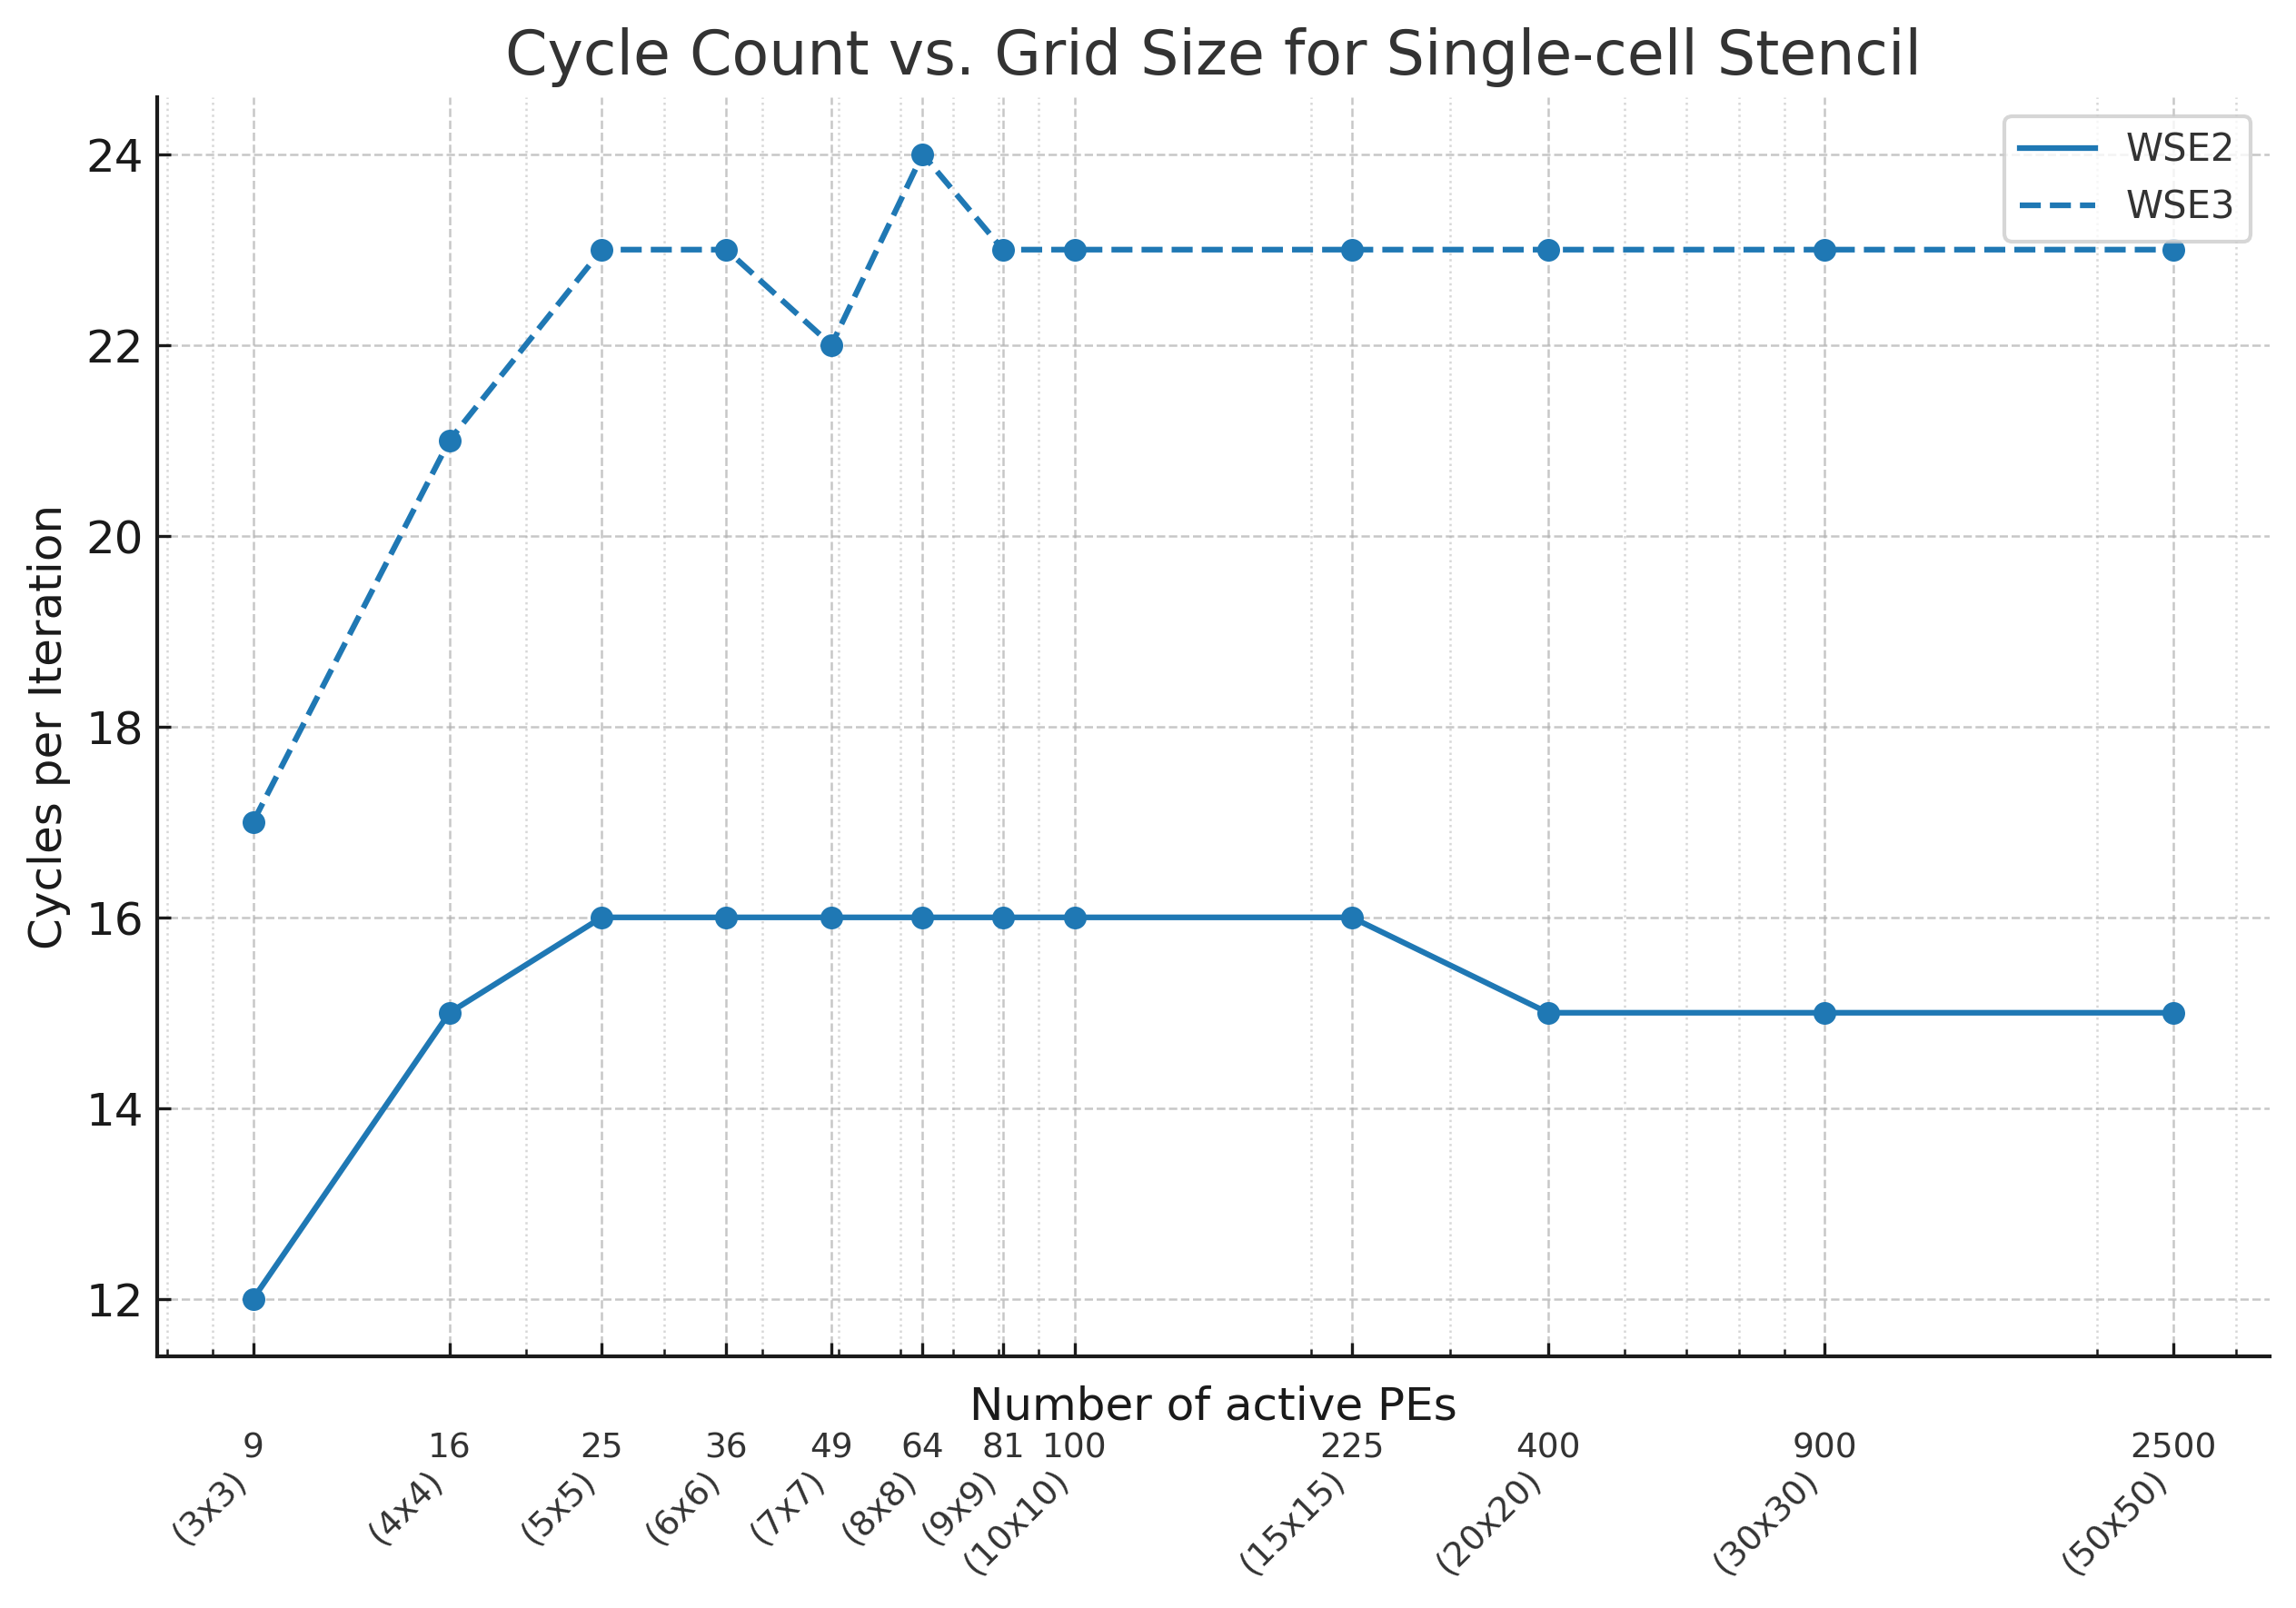
\includegraphics[width=\textwidth]{pe_overhead_non_tiled.png}
        \caption{Single-cell implementation}
        \label{fig:pe_overhead_non_tiled}
    \end{subfigure}
    \hfill
    \begin{subfigure}[b]{0.48\textwidth}
        \centering
        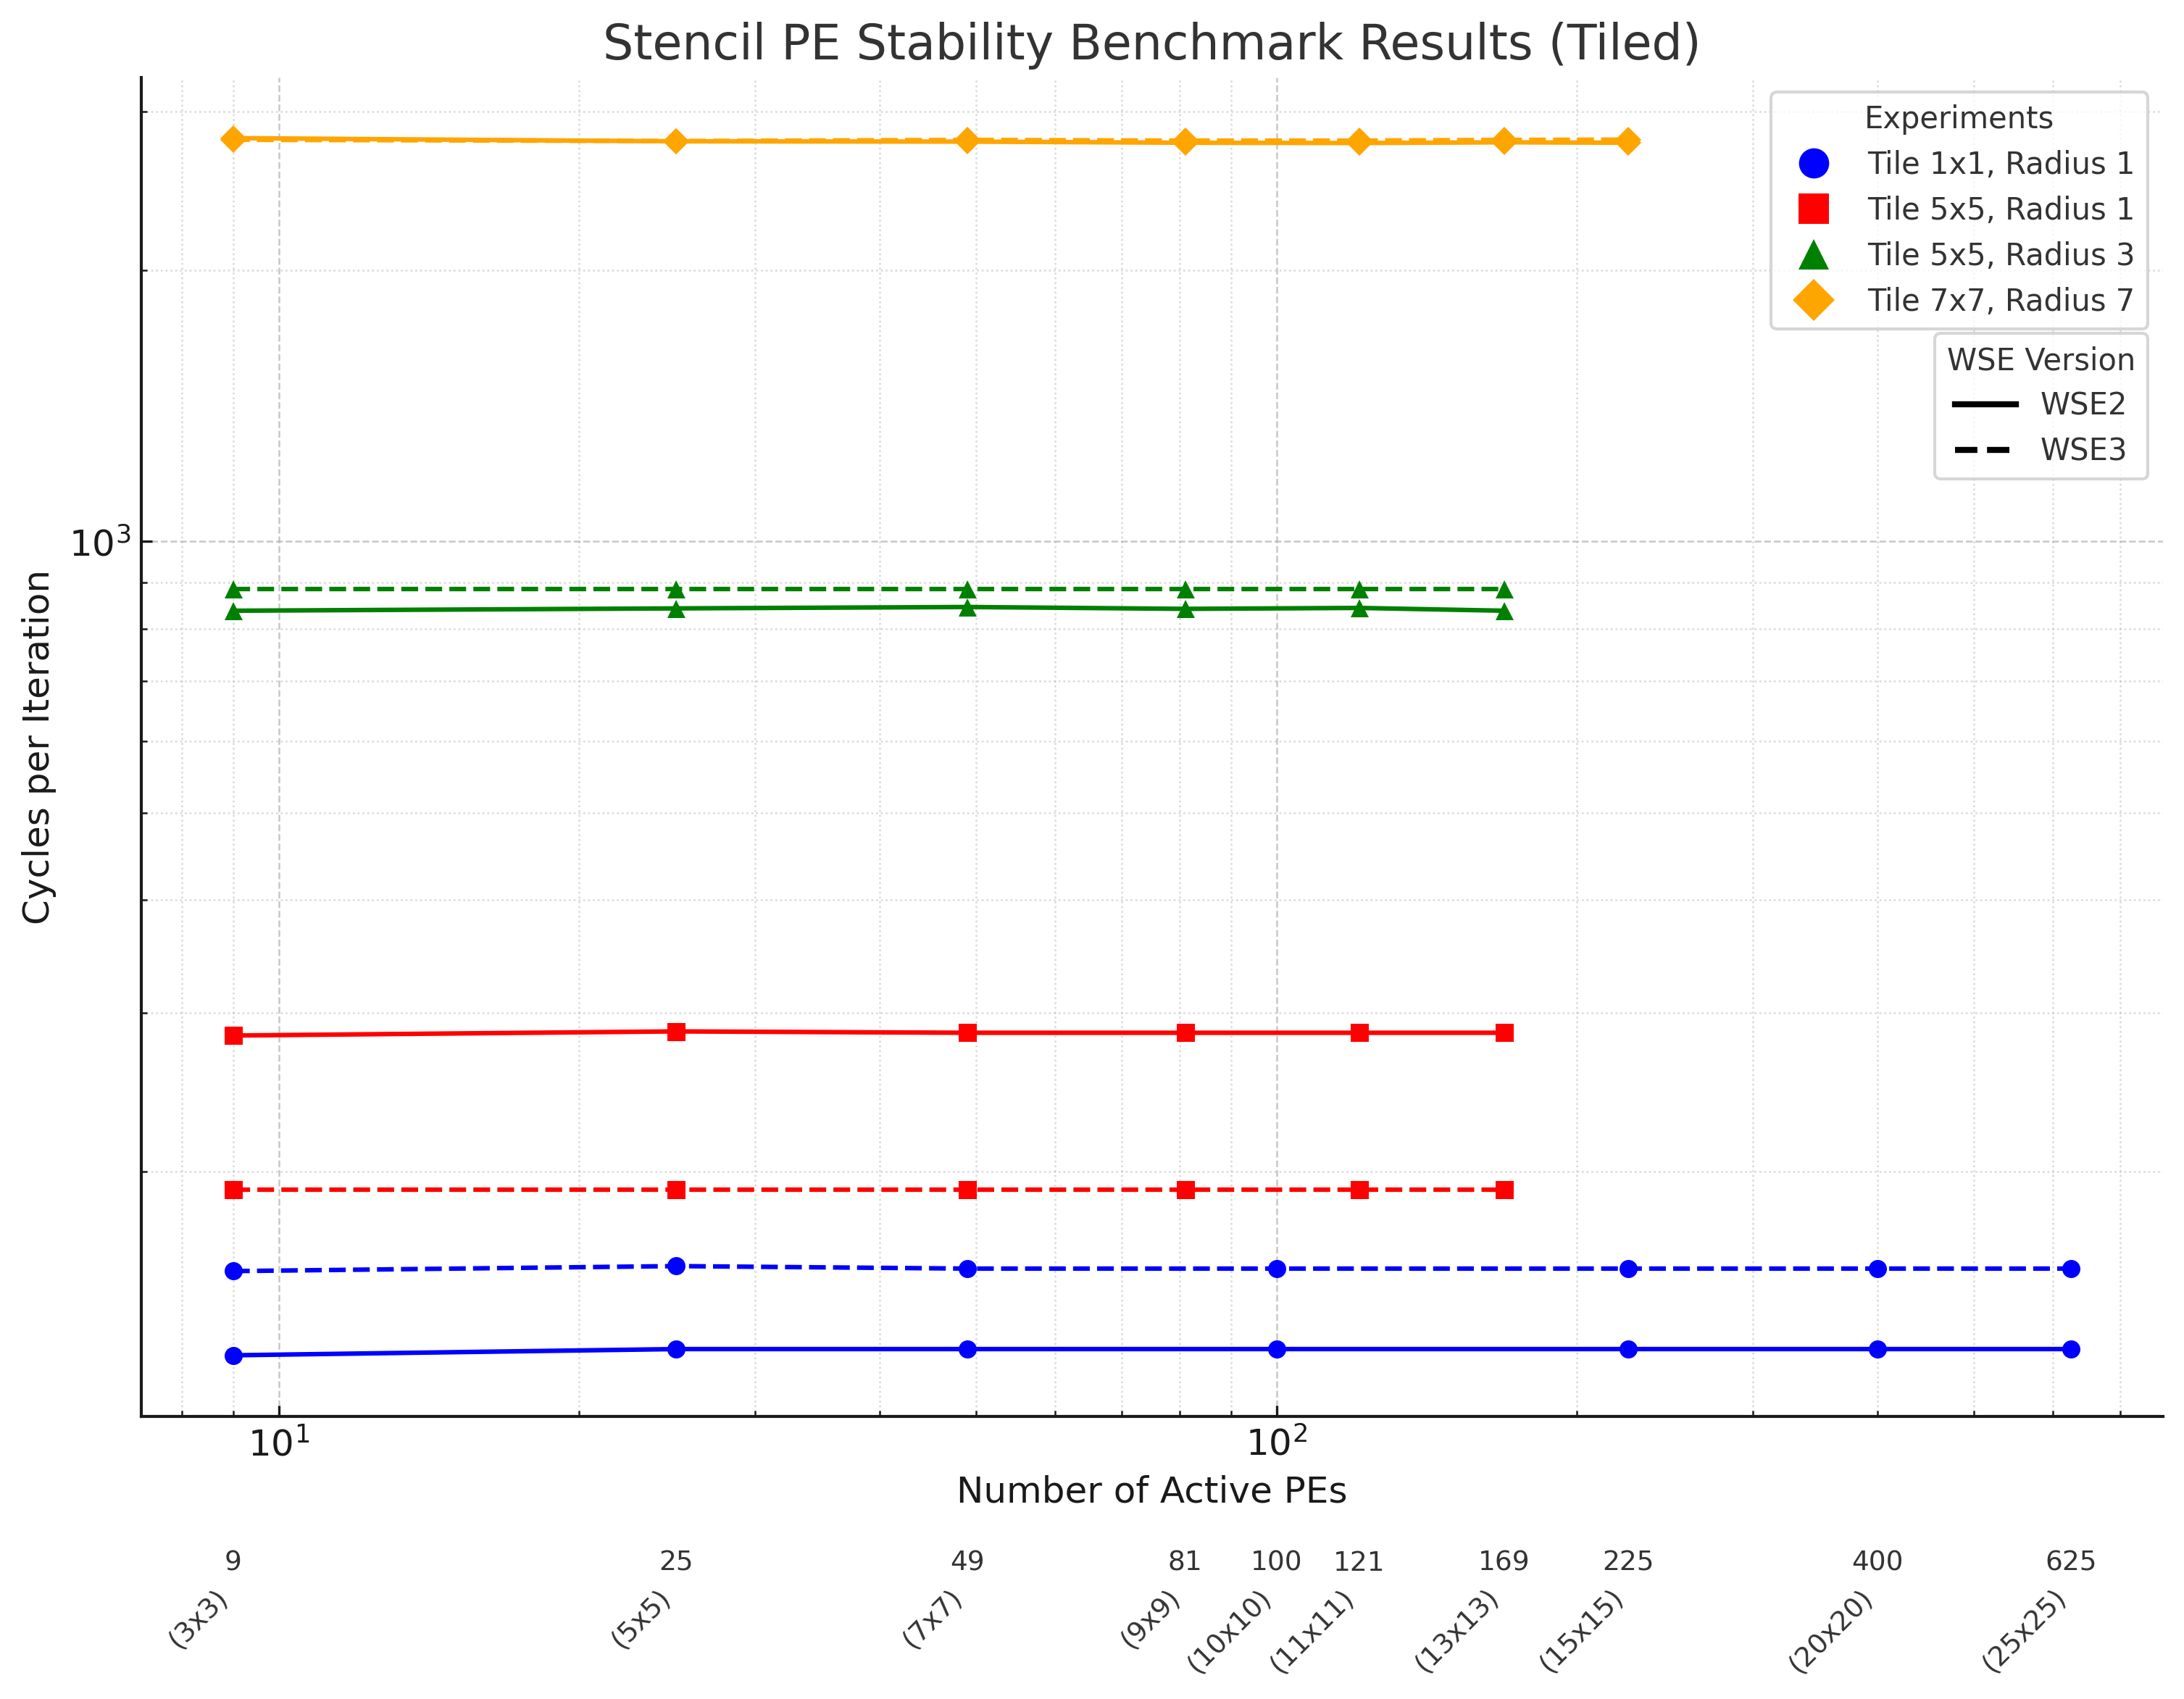
\includegraphics[width=\textwidth]{tiled_pe_stability.png}
        \caption{Tiled implementation}
        \label{fig:tiled_pe_stability}
    \end{subfigure}
    \caption{Cycle count per iteration versus the number of active \acp{pe} for (a) the single-cell and (b) the tiled implementation}
    \label{fig:pe_overhead}
\end{figure}

As shown in \autoref{fig:pe_overhead_non_tiled}, the performance of the single-cell implementation scales almost proportionally, with the cycle count remaining constant with minimal fluctuations regardless of the grid size. The one exception is the \numproduct{3 x 3} grid, which is significantly faster. We hypothesize this is an artifact of the experimental setup where only the single inner \ac{pe} is performing computation and does not need to synchronize with other computing neighbors, effectively eliminating any communication latency.
The tiled implementation doesn't show this behavior and fluctuates by no more than about 1.3\% on the \ac{wse}-3 across all tested grid sizes.
For all subsequent experiments, we ensure at least \numproduct{5 x 5} active \acp{pe}, which results in at least \numproduct{3 x 3} inner \acp{pe}, to avoid possible effects as observed for the single-cell implementation with a \numproduct{3 x 3} grid. 

\subsection{Iteration Stability}
\label{sec:stability_of_cycle_count_per_iteration}
For this experiment, we fix the grid size, tile size, and radius and run the simulation for different numbers of iterations to test whether the cycle count per iteration remains stable, which this experiment shows to be the case after two iterations of varying cycle count.
% For our single-cell implementaion and a grid size of \numproduct{10 x 10}, the cycle count per iteration is $16\pm1$ on \ac{wse}-2 and $23\pm1$ on \ac{wse}-3.
% For a grid of \numproduct{10 x 10}, a tile size of \numproduct{1 x 1} and radius 1, the tiled algorithm achieves $127\pm0$ cycles per iteration on \ac{wse}-2 and $156\pm1$ cycles per iteration on \ac{wse}-3.
% A larger problem size with a grid of 100x100, tile size of 10x10 and radius 5, results in a cycle count per iteration of $3353\pm20$ on \ac{wse}-2 and $3377\pm5$ on \ac{wse}-3.
Because of the higher fluctuations in cycle count in the first two iterations, we measure the cycle count in the following experiments as an average of the 3rd and 4th iteration.
\begin{figure}[h]
    \centering
    \begin{subfigure}[b]{0.48\textwidth}
        \centering
        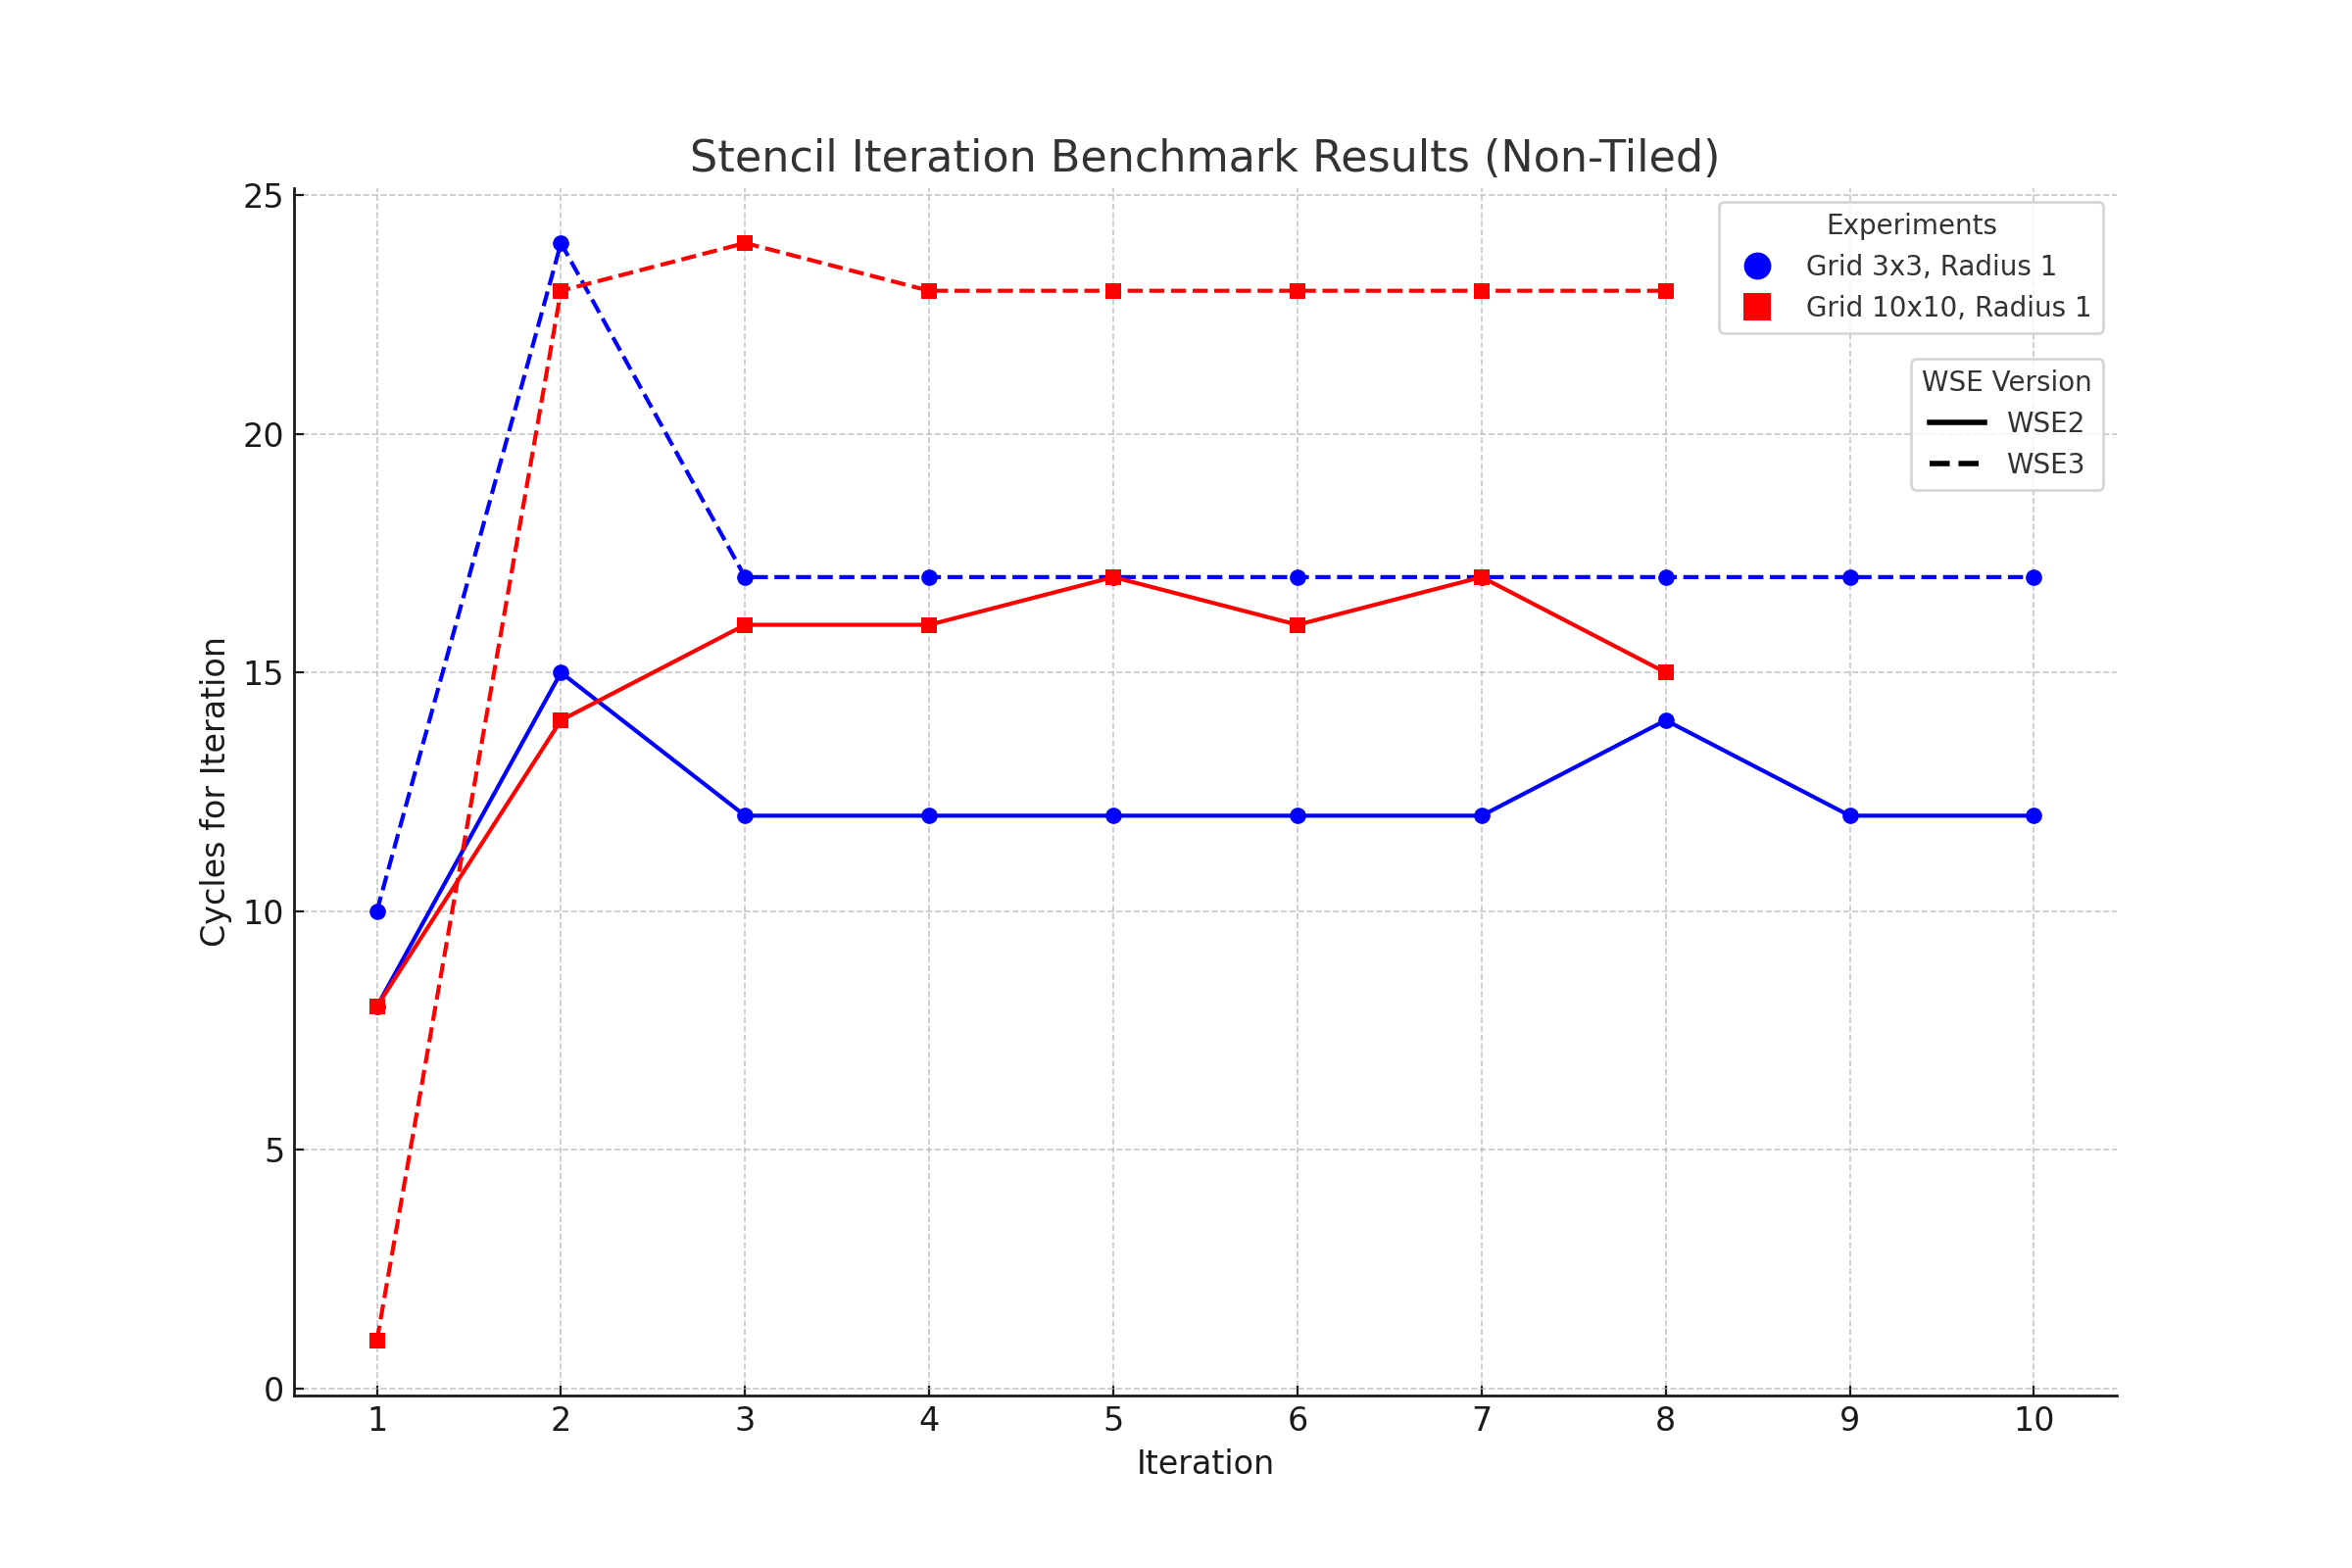
\includegraphics[width=\textwidth]{non_tiled_iteration_stability.png}
        \caption{Single-cell implementation}
        \label{fig:non_tiled_iteration_stability}
    \end{subfigure}
    \hfill
    \begin{subfigure}[b]{0.48\textwidth}
        \centering
        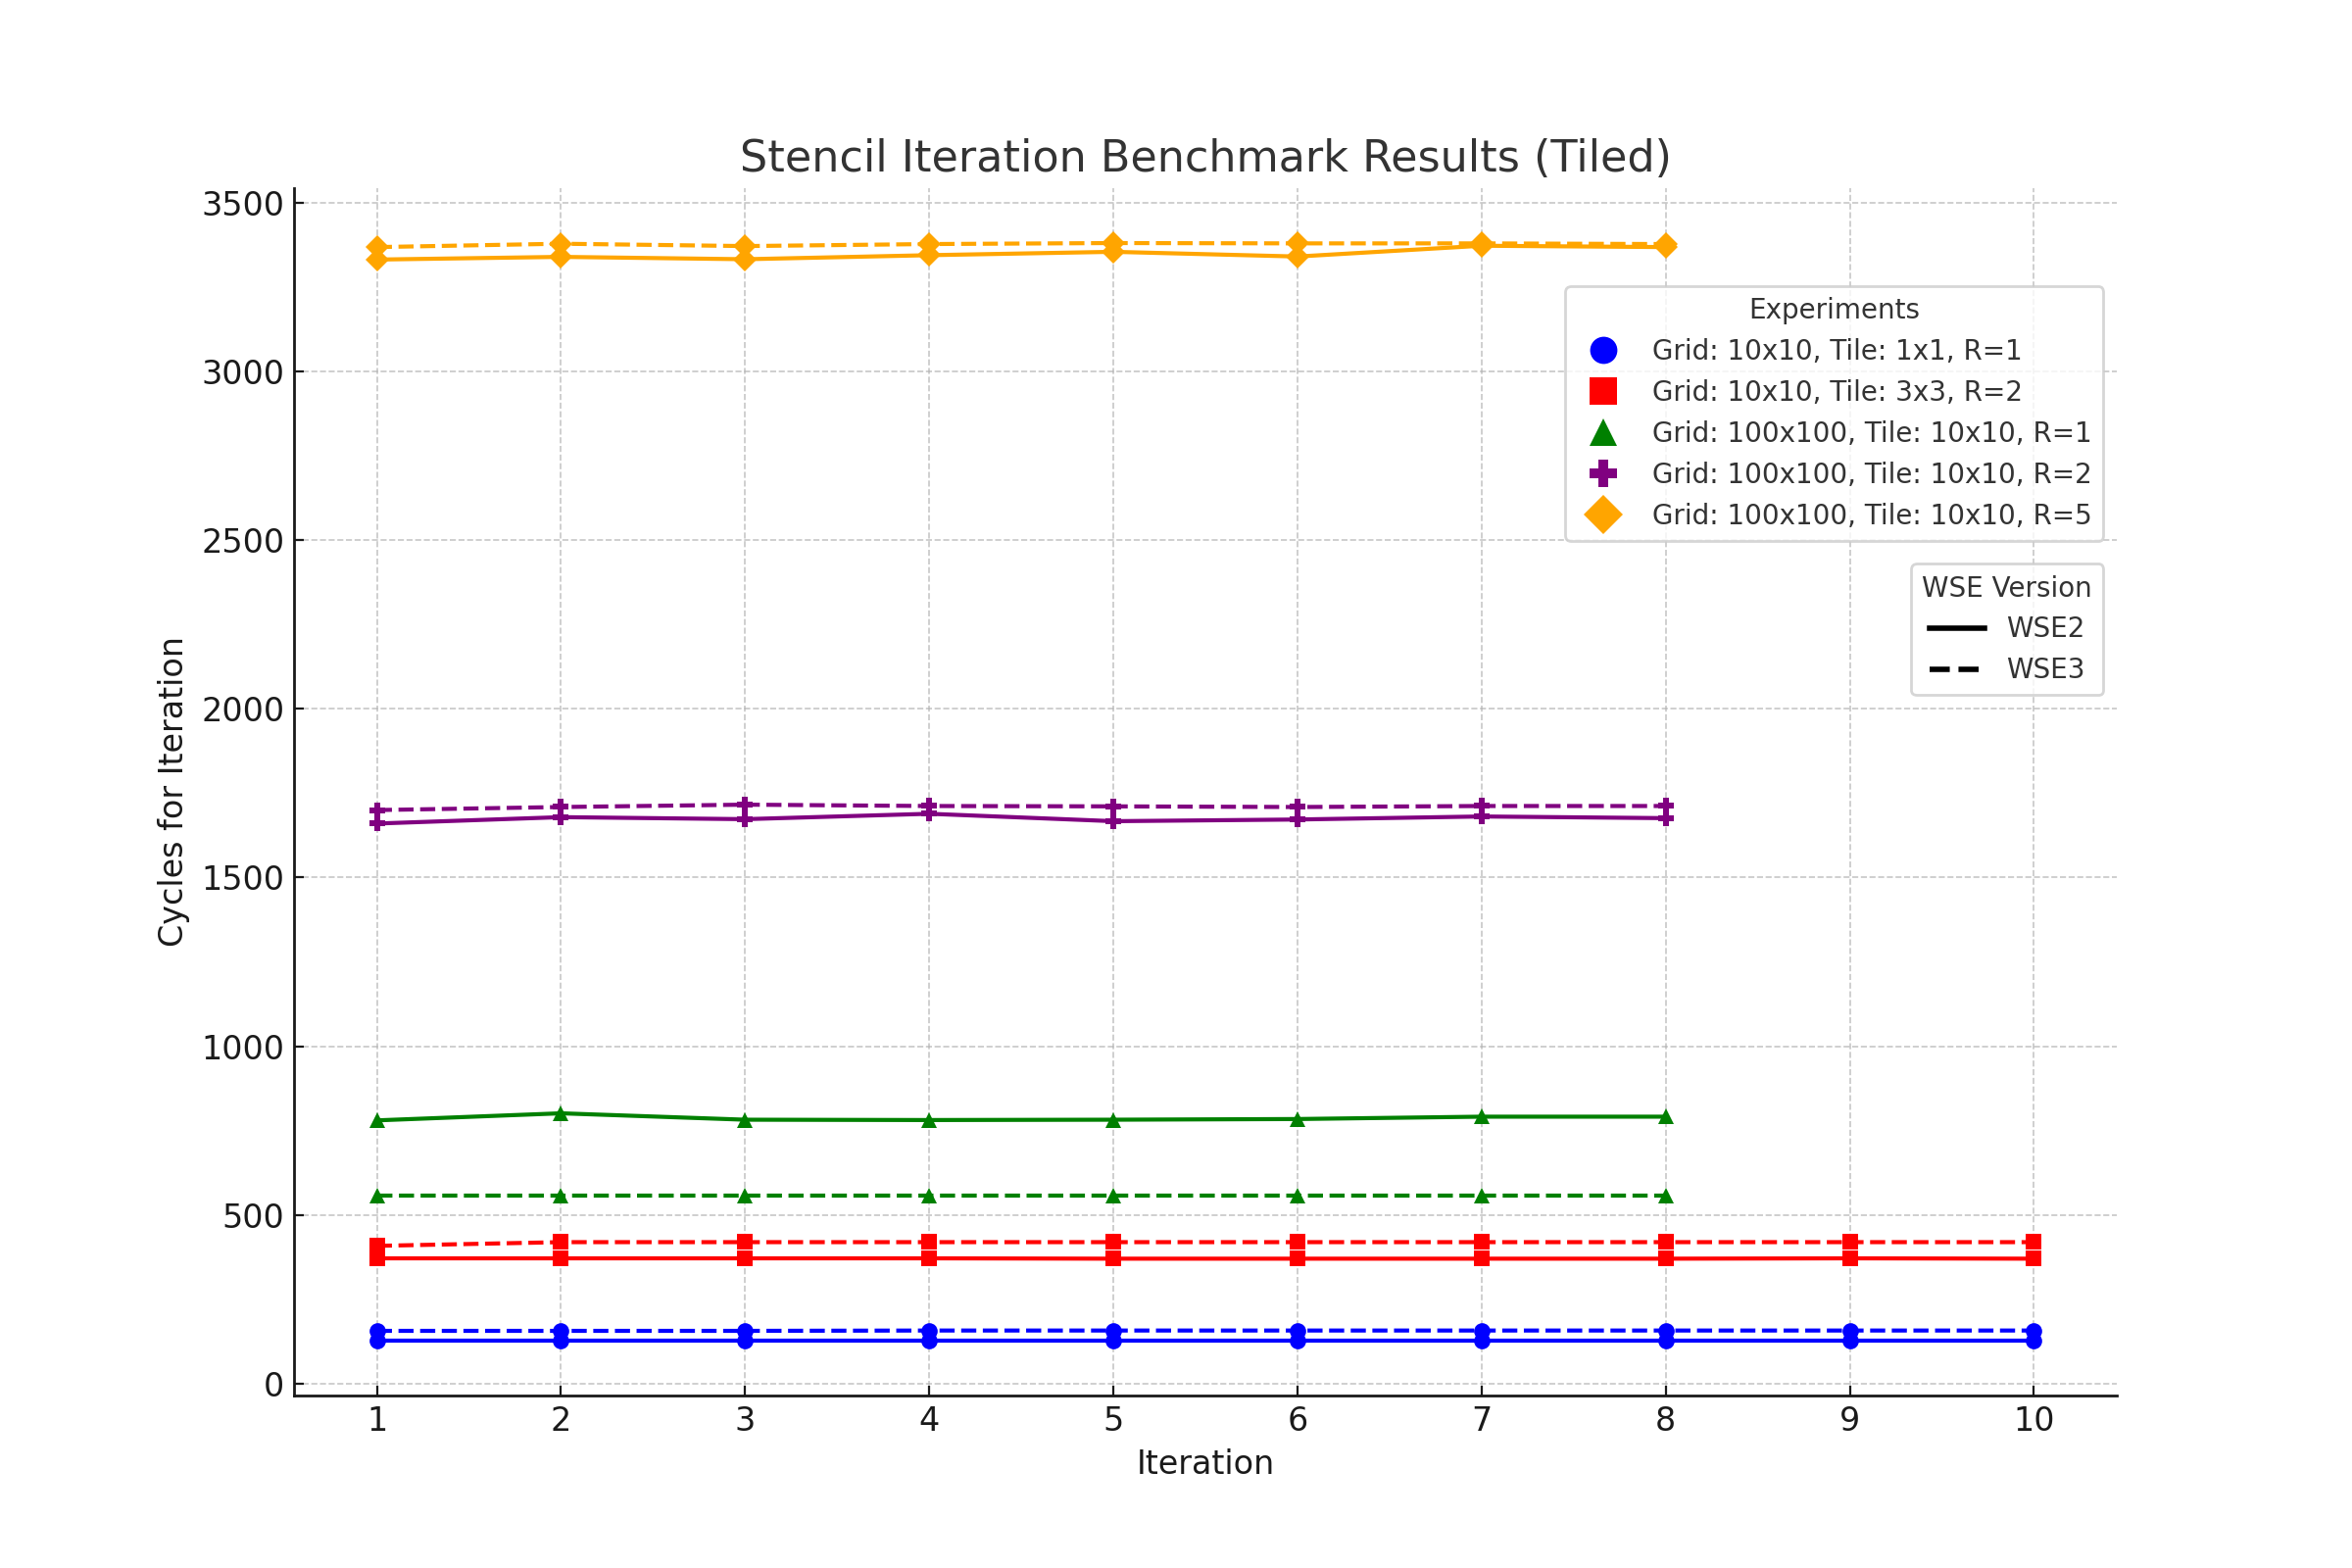
\includegraphics[width=\textwidth]{tiled_iteration_stability.png}
        \caption{Tiled implementation}
        \label{fig:tiled_iteration_stability}
    \end{subfigure}
    \caption{Cycle count per iteration for single-cell and tiled implementations}
    \label{fig:iteration_stability}
\end{figure}

\subsection{Theoretical Performance Model}
\label{sec:perf_model_validation}
We now analyze the impact of tiling and radius, both in our theoretical performance model and with experiments using our implementation.
\begin{figure}[h]
    \centering
    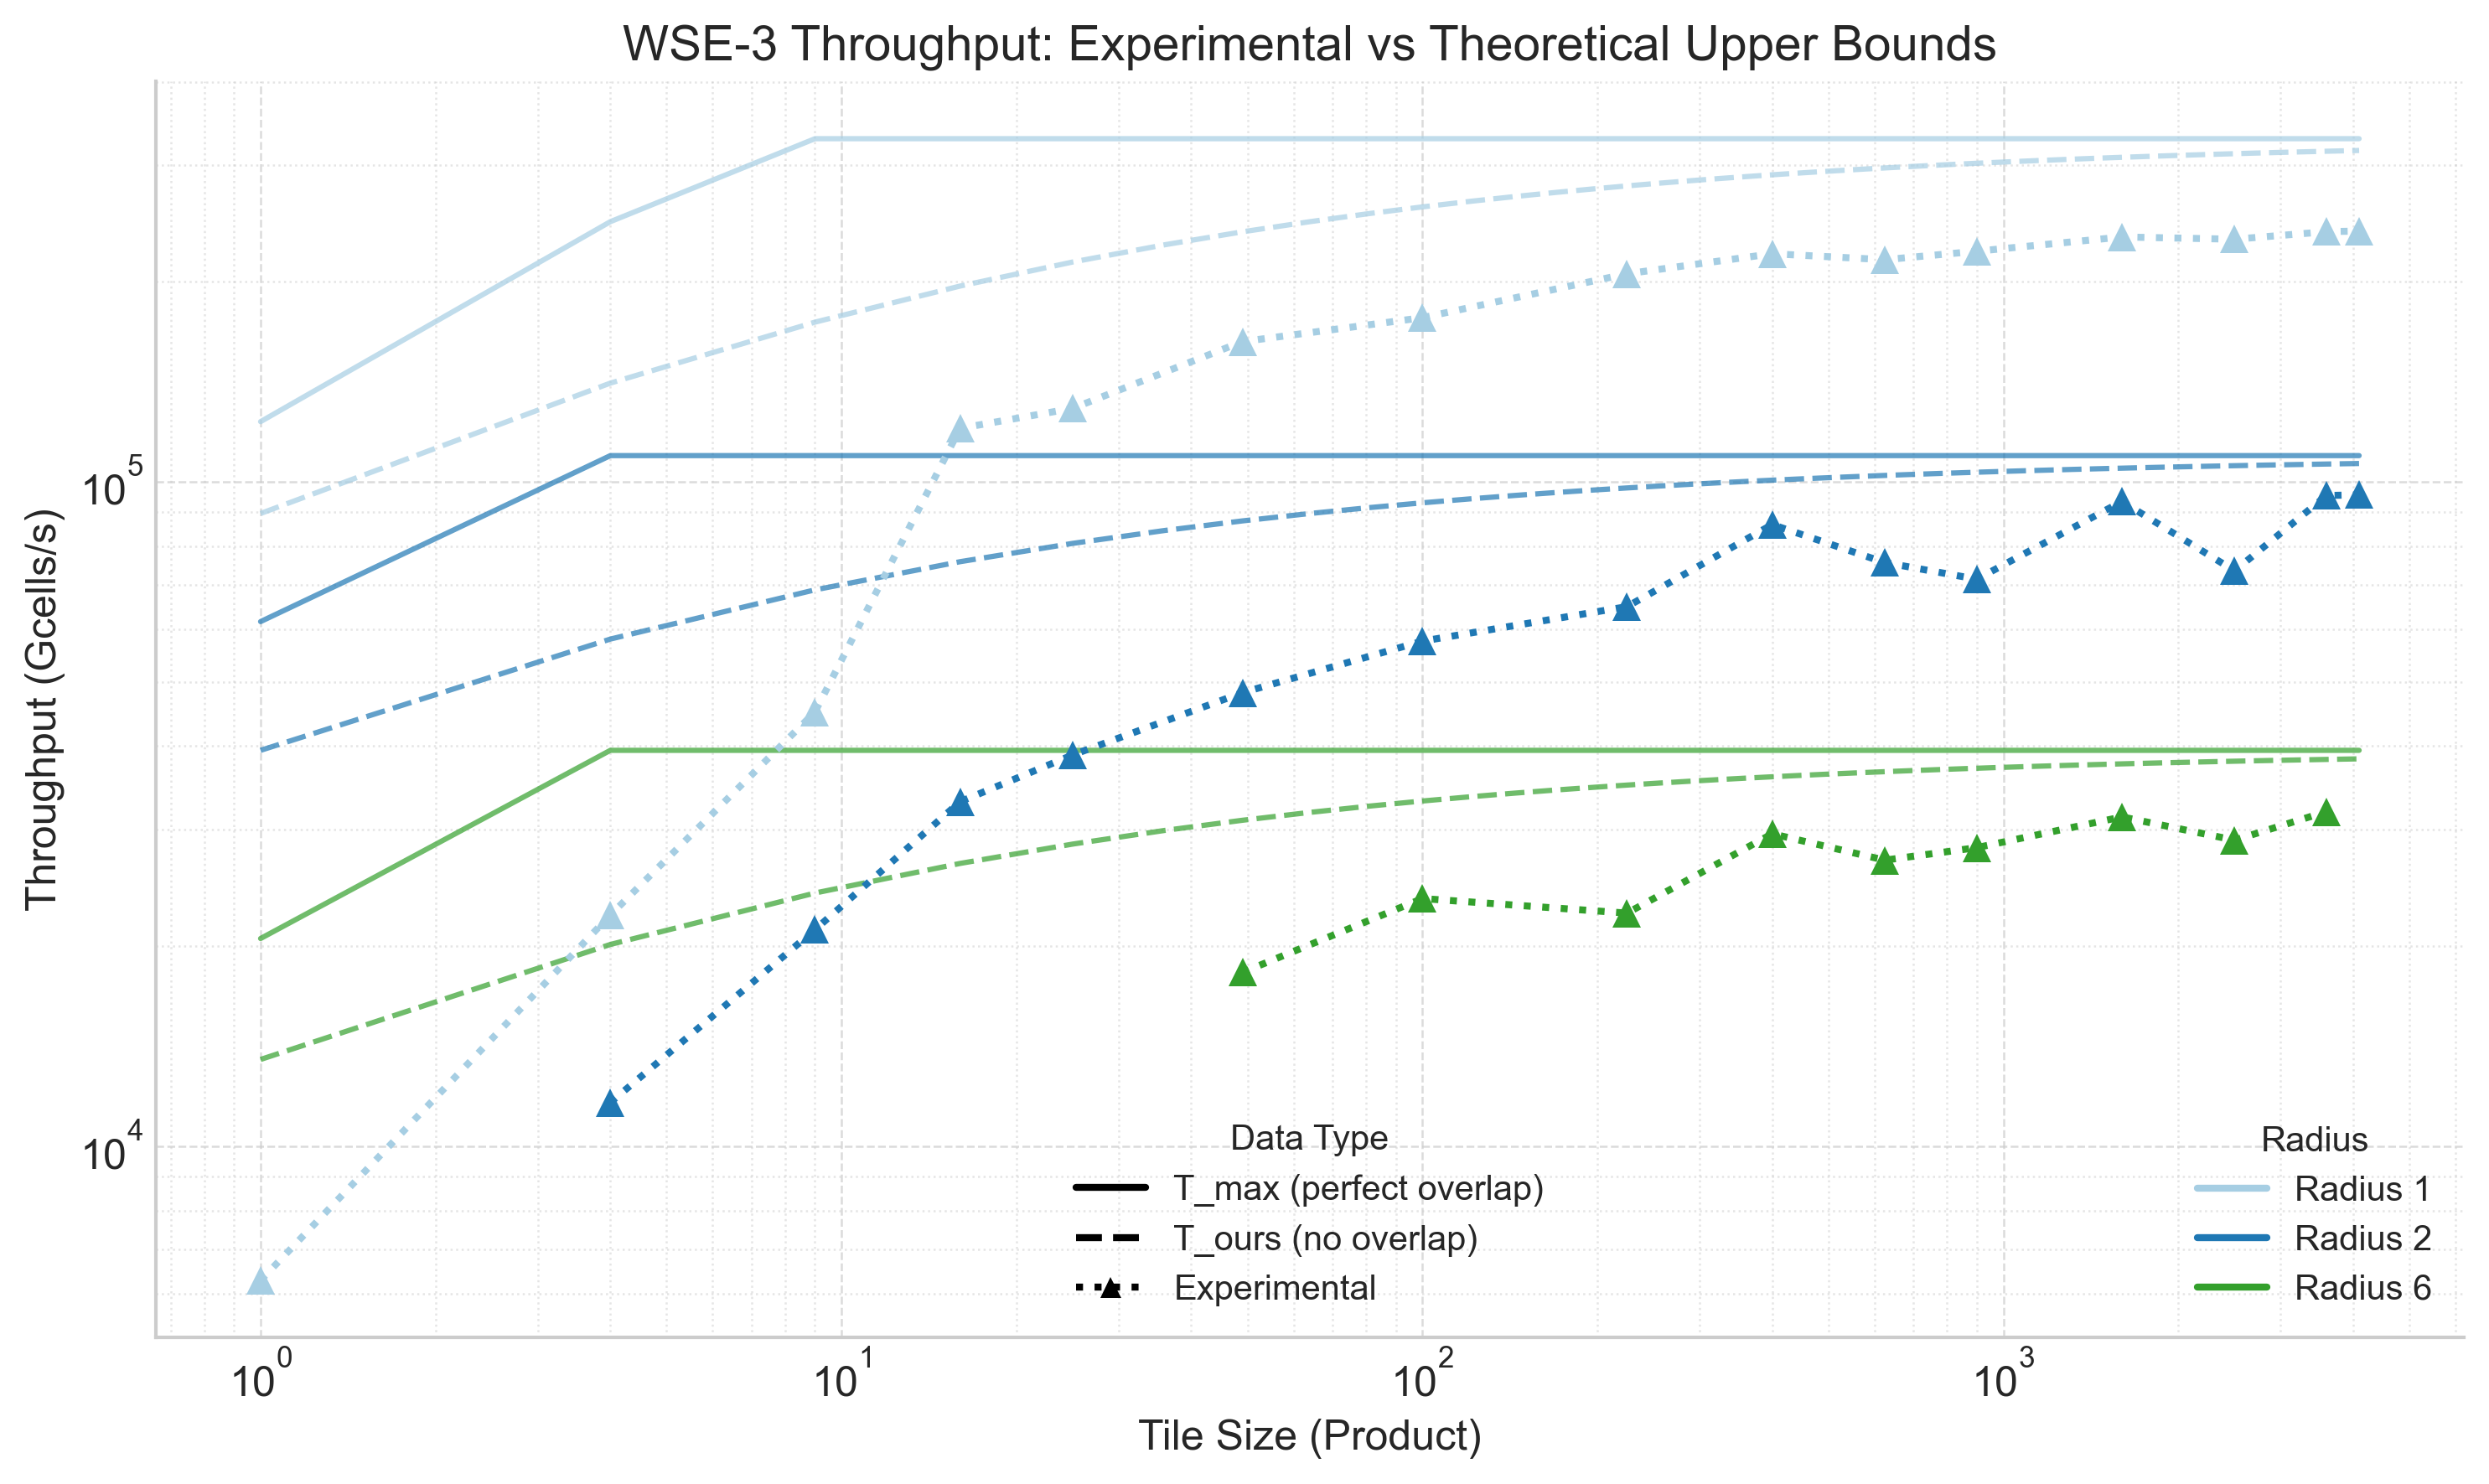
\includegraphics[width=0.7\linewidth]{throughput_comparison_wse3.png}
    \caption{Throughput comparison showing theoretical bounds ($T_{ideal}$, $T_{sequential}$) and measured performance for different radii and tile sizes}
    \label{fig:throughput_comparison_wse3}
\end{figure}
We can see that the throughput of the theoretical model scales almost proportionally to the inverse of the radius, and while the ideal model has a constant throughput for large enough tile sizes, the throughput of the sequential model increases as the tile sizes get larger.
However, the difference between $T_{ideal}$ and $T_{sequential}$ decreases as the tile size increases. This is because the term for the computation cycles $C_{comp}$ scales with the area of the tile $t_w \times t_h$, while the communication term $C_{comm}$ only scales with the length of the border $t_w+t_h$, making it less significant for larger tiles.

Our implementation gets relatively close to the possible throughput modeled by $T_{ideal}$ and $T_{sequential}$ for large tile sizes with up to 87.3\% or 89.7\% respectively, whereas it is below 10\% for small tile sizes. This can be explained by constant overhead per iteration that emerges from loading \acp{dsd} into \acp{dsr}, activating tasks, and communication latency.

More interesting are the gaps between our implementation and $T_{sequential}$ even for large tile sizes. These must be attributed to factors that scale with $C_{comp}$. For the r1-optimized implementation, the gap is significantly larger, with our implementation reaching only 75\% of the $T_{sequential}$ model. We assume this is the case because the implementation mainly uses \texttt{@fadds} instructions that support a \ac{simd} width of four, which is never reached by our implementation. The general tiled implementation, on the other hand, uses only \texttt{@fmacs} and \texttt{@fmuls} instructions that have a \ac{simd} width of one, which our implementation mostly does reach.

There is relatively high jitter in the throughput for radius 2. We don't know why this is the case, but speculate that bank conflicts might occur for certain buffer sizes, limiting the \texttt{@fmacs} and \texttt{@fmuls} to less than one per cycle.

The largest tile size we could test is \numproduct{64 x 64} cells with a radius of up to three, resulting in a theoretically possible problem size containing up to \num{3.6e9} elements on the \ac{wse}-3. The limiting factor is the available memory per \ac{pe} of \qty{48}{\kilo\byte}. Increasing the radius reduces the maximum possible tile size as the halo regions needed to store the values from the neighboring \acp{pe} also get larger.

\section{Comparative Performance Analysis}
Comparing our implementation against implementations optimized for traditional \ac{hpc} architectures lets us assess for which parameters it is most beneficial. We also compare our specialized single-cell implementation to the tiled implementation.  

\subsection{Specialized vs. General Kernel}
The single-cell implementation is a heavily optimized implementation for the special case of only one element per \ac{pe}. It is useful for situations where the problem size is smaller than the physical dimensions of the \ac{wse}. In contrast to the tiled implementation, it doesn't require any runtime \ac{dsd} to \ac{dsr} transfers, asynchronous communication, or multiple tasks. These aspects cause most of the overhead in the tiled implementation. Furthermore, it implements overlap between communication and computation, which makes it significantly faster than the r1-optimized version of the tiled implementation, specifically achieving an 8x improvement in throughput on the \ac{wse}-2 and a 7x improvement on the \ac{wse}-3.
\begin{figure}[h]
    \centering
    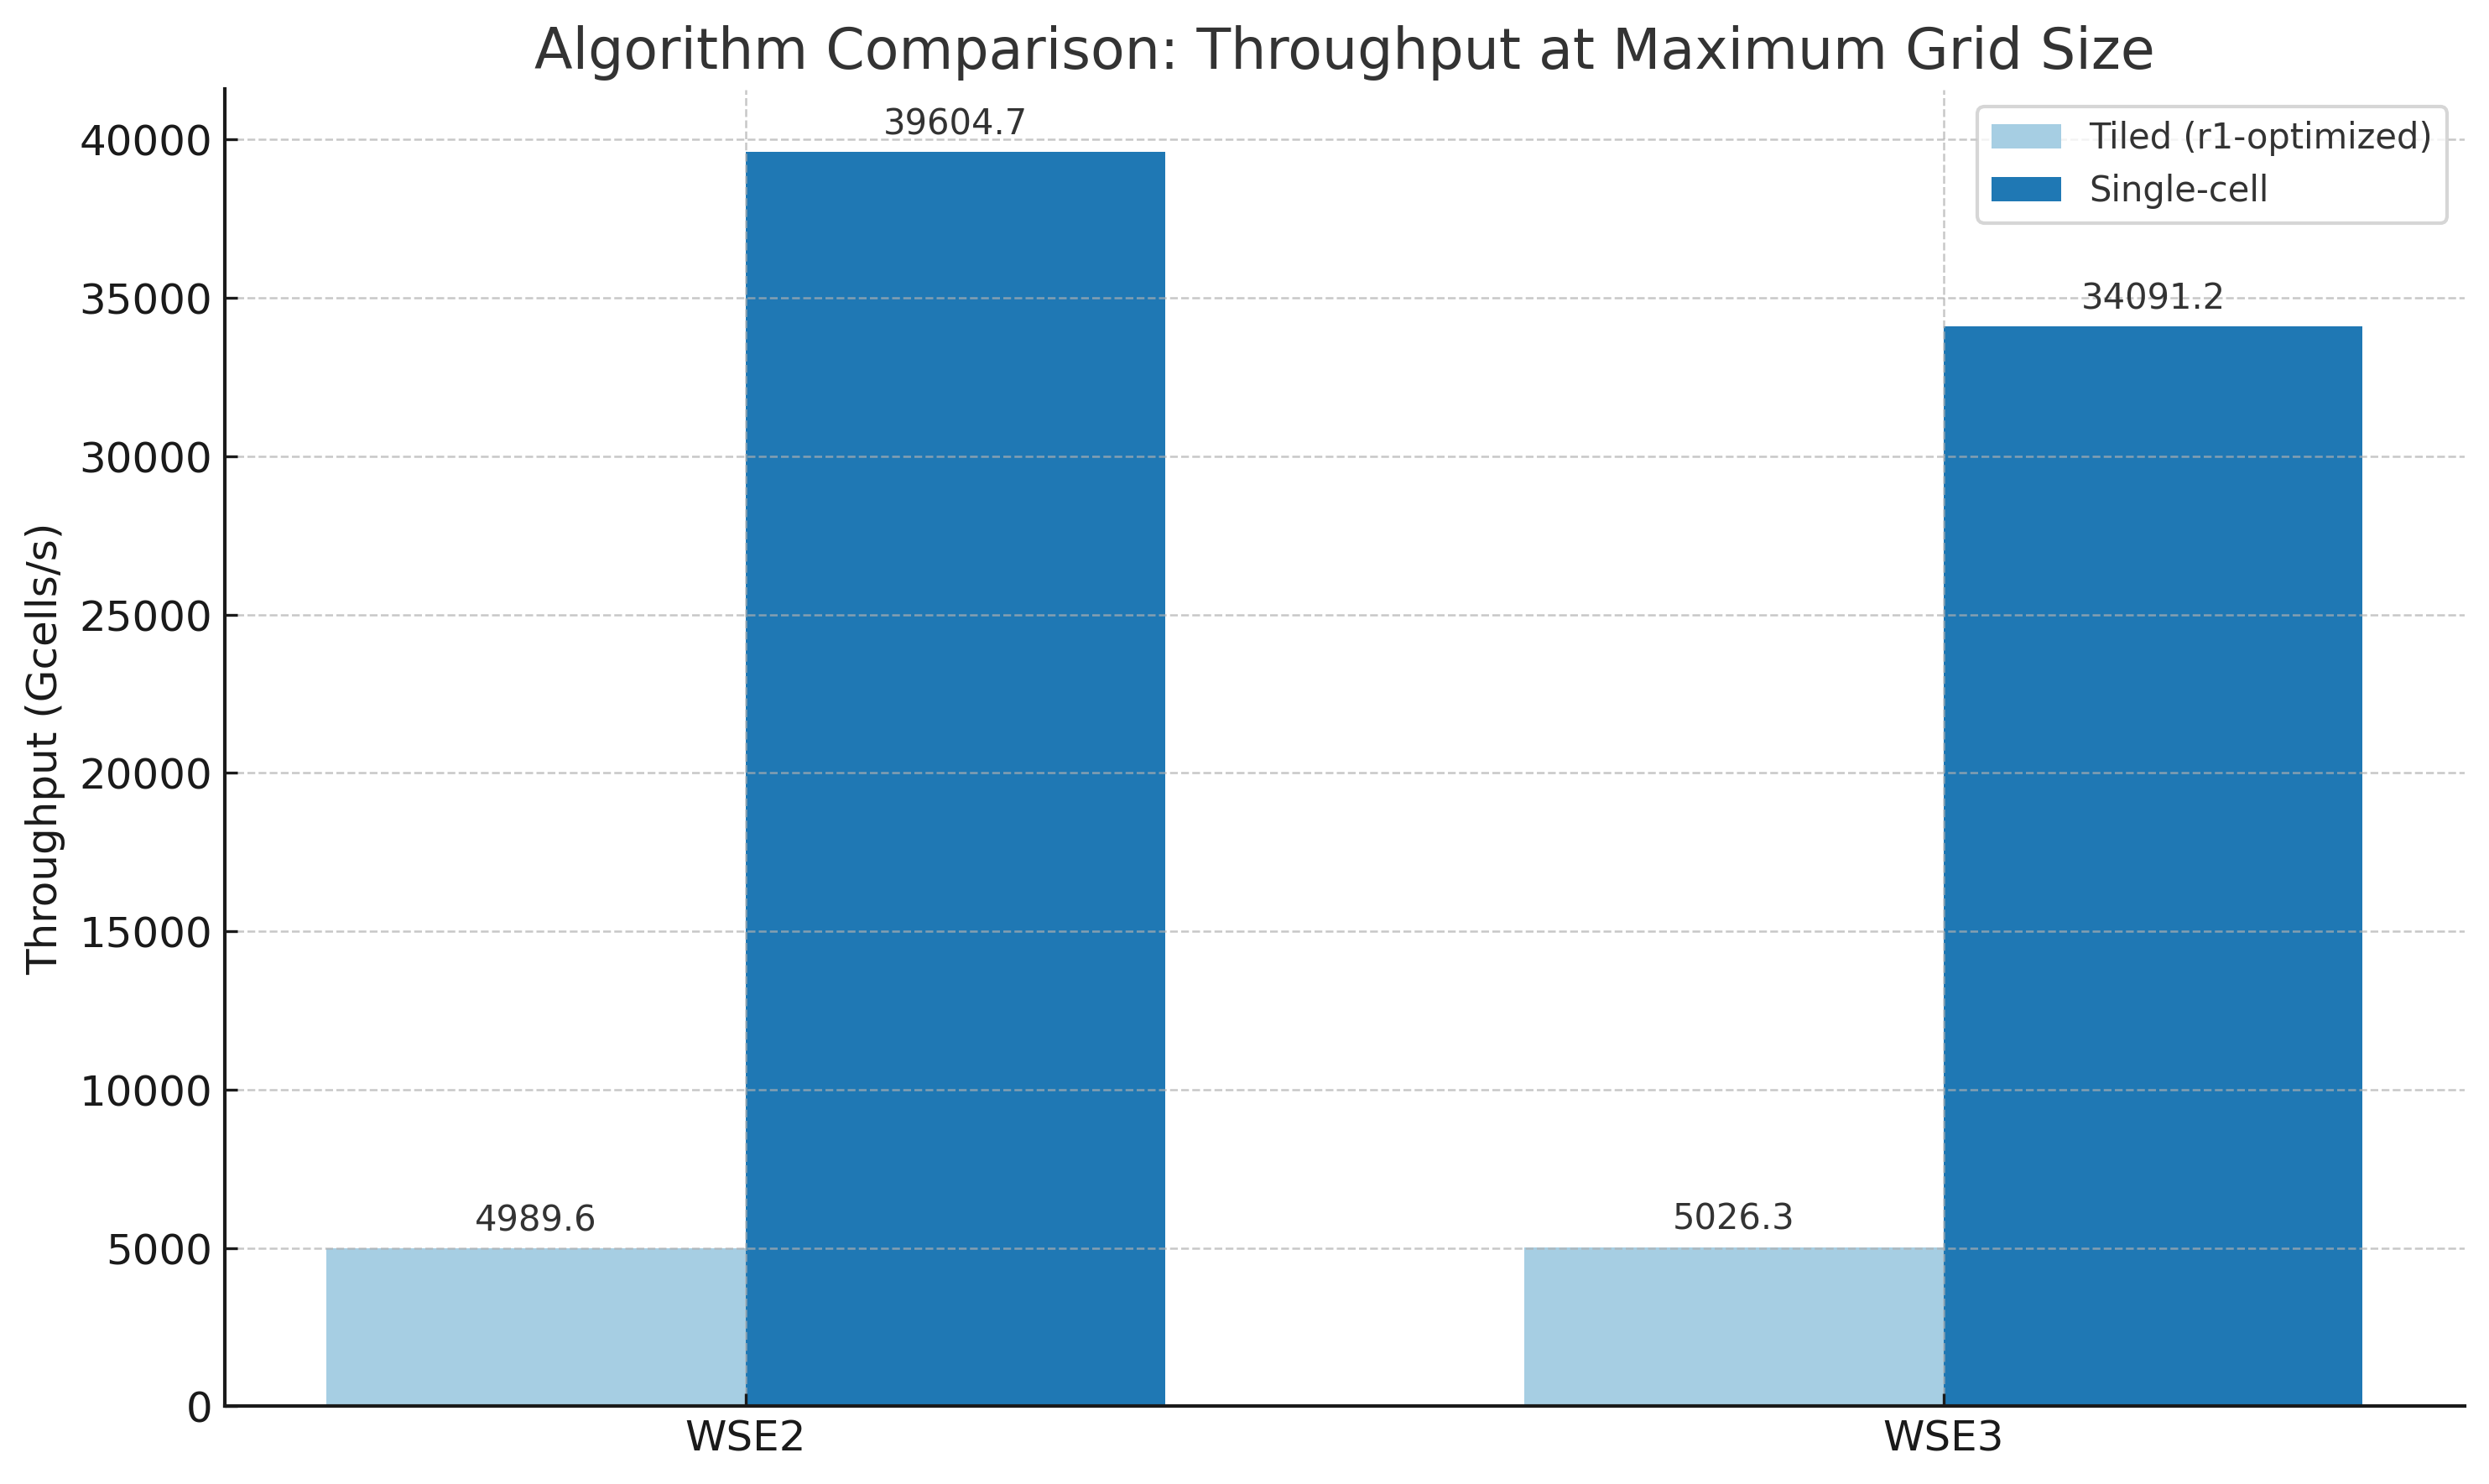
\includegraphics[width=0.7\linewidth]{algo_comparison.png}
    \caption{Throughput comparison of the specialized single-cell and the r1-optimized tiled implementations for a radius-1 stencil on \ac{wse}-2 and \ac{wse}-3}
    \label{fig:algo_comparison}
\end{figure}

\subsection{Comparison with \ac{hpc} Architectures}
To quantify the advantage of the \ac{wse} architecture, we conducted two more experiments comparing the performance of our stencil implementation with highly optimized Devito implementations for \ac{cpu} and \ac{gpu}. 

To enable a fair evaluation, we implemented the same 2D star-shaped stencil using the Devito framework (version 4.8.19) in Python (version 3.12.11), using the same symmetric, constant coefficients that we used for the experiments on the \ac{wse}.
Devito automatically optimizes and compiles the code for various hardware targets.
For the \ac{cpu} experiments, we used a system equipped with two AMD EPYC 9554 64-Core processors. For the \ac{gpu} experiments, we employed a system with one NVIDIA H100 SXM 80GB \ac{gpu}, configured Devito to use the OpenACC backend, and compiled with the nvc compiler (version 25.5) under CUDA driver version 12.8. All \ac{cpu} and \ac{gpu} experiments ran in the Vast.ai cloud.
Steady-state performance was obtained by first running an untimed warm-up of $N$ iterations (triggering JIT compilation, allocations, and data transfers) and then timing a second run of the same $N$ iterations with all data already resident on the \ac{cpu} or \ac{gpu}.
This was done for grids with a total size of $10^i$ for $i \in \{4..9\}$ and $r \in \{1..6\}$.

To compare these results with our implementation, we started from each grid size and calculated the minimal tile size that would allow the entire grid to fit on the \ac{wse}-3.
We then ran simulations with this tile size for radii 1 to 6 and extrapolated the full-system throughput assuming perfect weak scaling. Furthermore, we added the throughput that the single-cell implementation could achieve on the \ac{wse}-3 where the problem size is smaller than the physical dimensions of the \ac{wse}.

In all experiments, we strictly used powers of 10 for the grid dimensions, sometimes resulting in rectangular grids (e.g., \numproduct{1e3 x 1e4} instead of \numproduct{\sqrt{1e7} x \sqrt{1e7}}). The required tile size ($t_w \times t_h$) for a given grid of size $G_w \times G_h$ on a \ac{wse} with physical dimensions $P_w \times P_h$ is determined by:
\begin{equation}
    t_w = \left\lceil \frac{G_w}{P_w} \right\rceil, \quad t_h = \left\lceil \frac{G_h}{P_h} \right\rceil
\end{equation}

To map a rectangular grid of $10^3\times 10^4$ elements onto the \ac{wse}-3 with its dimensions of \numproduct{762 x 1176} \acp{pe}, we can calculate the tile size in two possible ways. Mapping the grid's width to the \ac{wse}'s width results in a tile width of $\left\lceil \frac{1000}{762} \right\rceil = 2$ and a tile height of $\left\lceil \frac{10000}{1176} \right\rceil = 9$. However, mapping the grid's width to the \ac{wse}'s height is more efficient, yielding a tile width of $\left\lceil \frac{1000}{1176} \right\rceil = 1$ and a tile height of $\left\lceil \frac{10000}{762} \right\rceil = 14$. To minimize the total tile area and therefore the per-\ac{pe} workload, we always chose the smaller configuration of $1 \times 14$. It is important to note that due to the radius constraint from \autoref{eq:radius_constraint}, the shorter dimension of the tile must be at least as large as the radius, so the effective tile size was adjusted accordingly if necessary.

\begin{figure}[h]
    \centering
    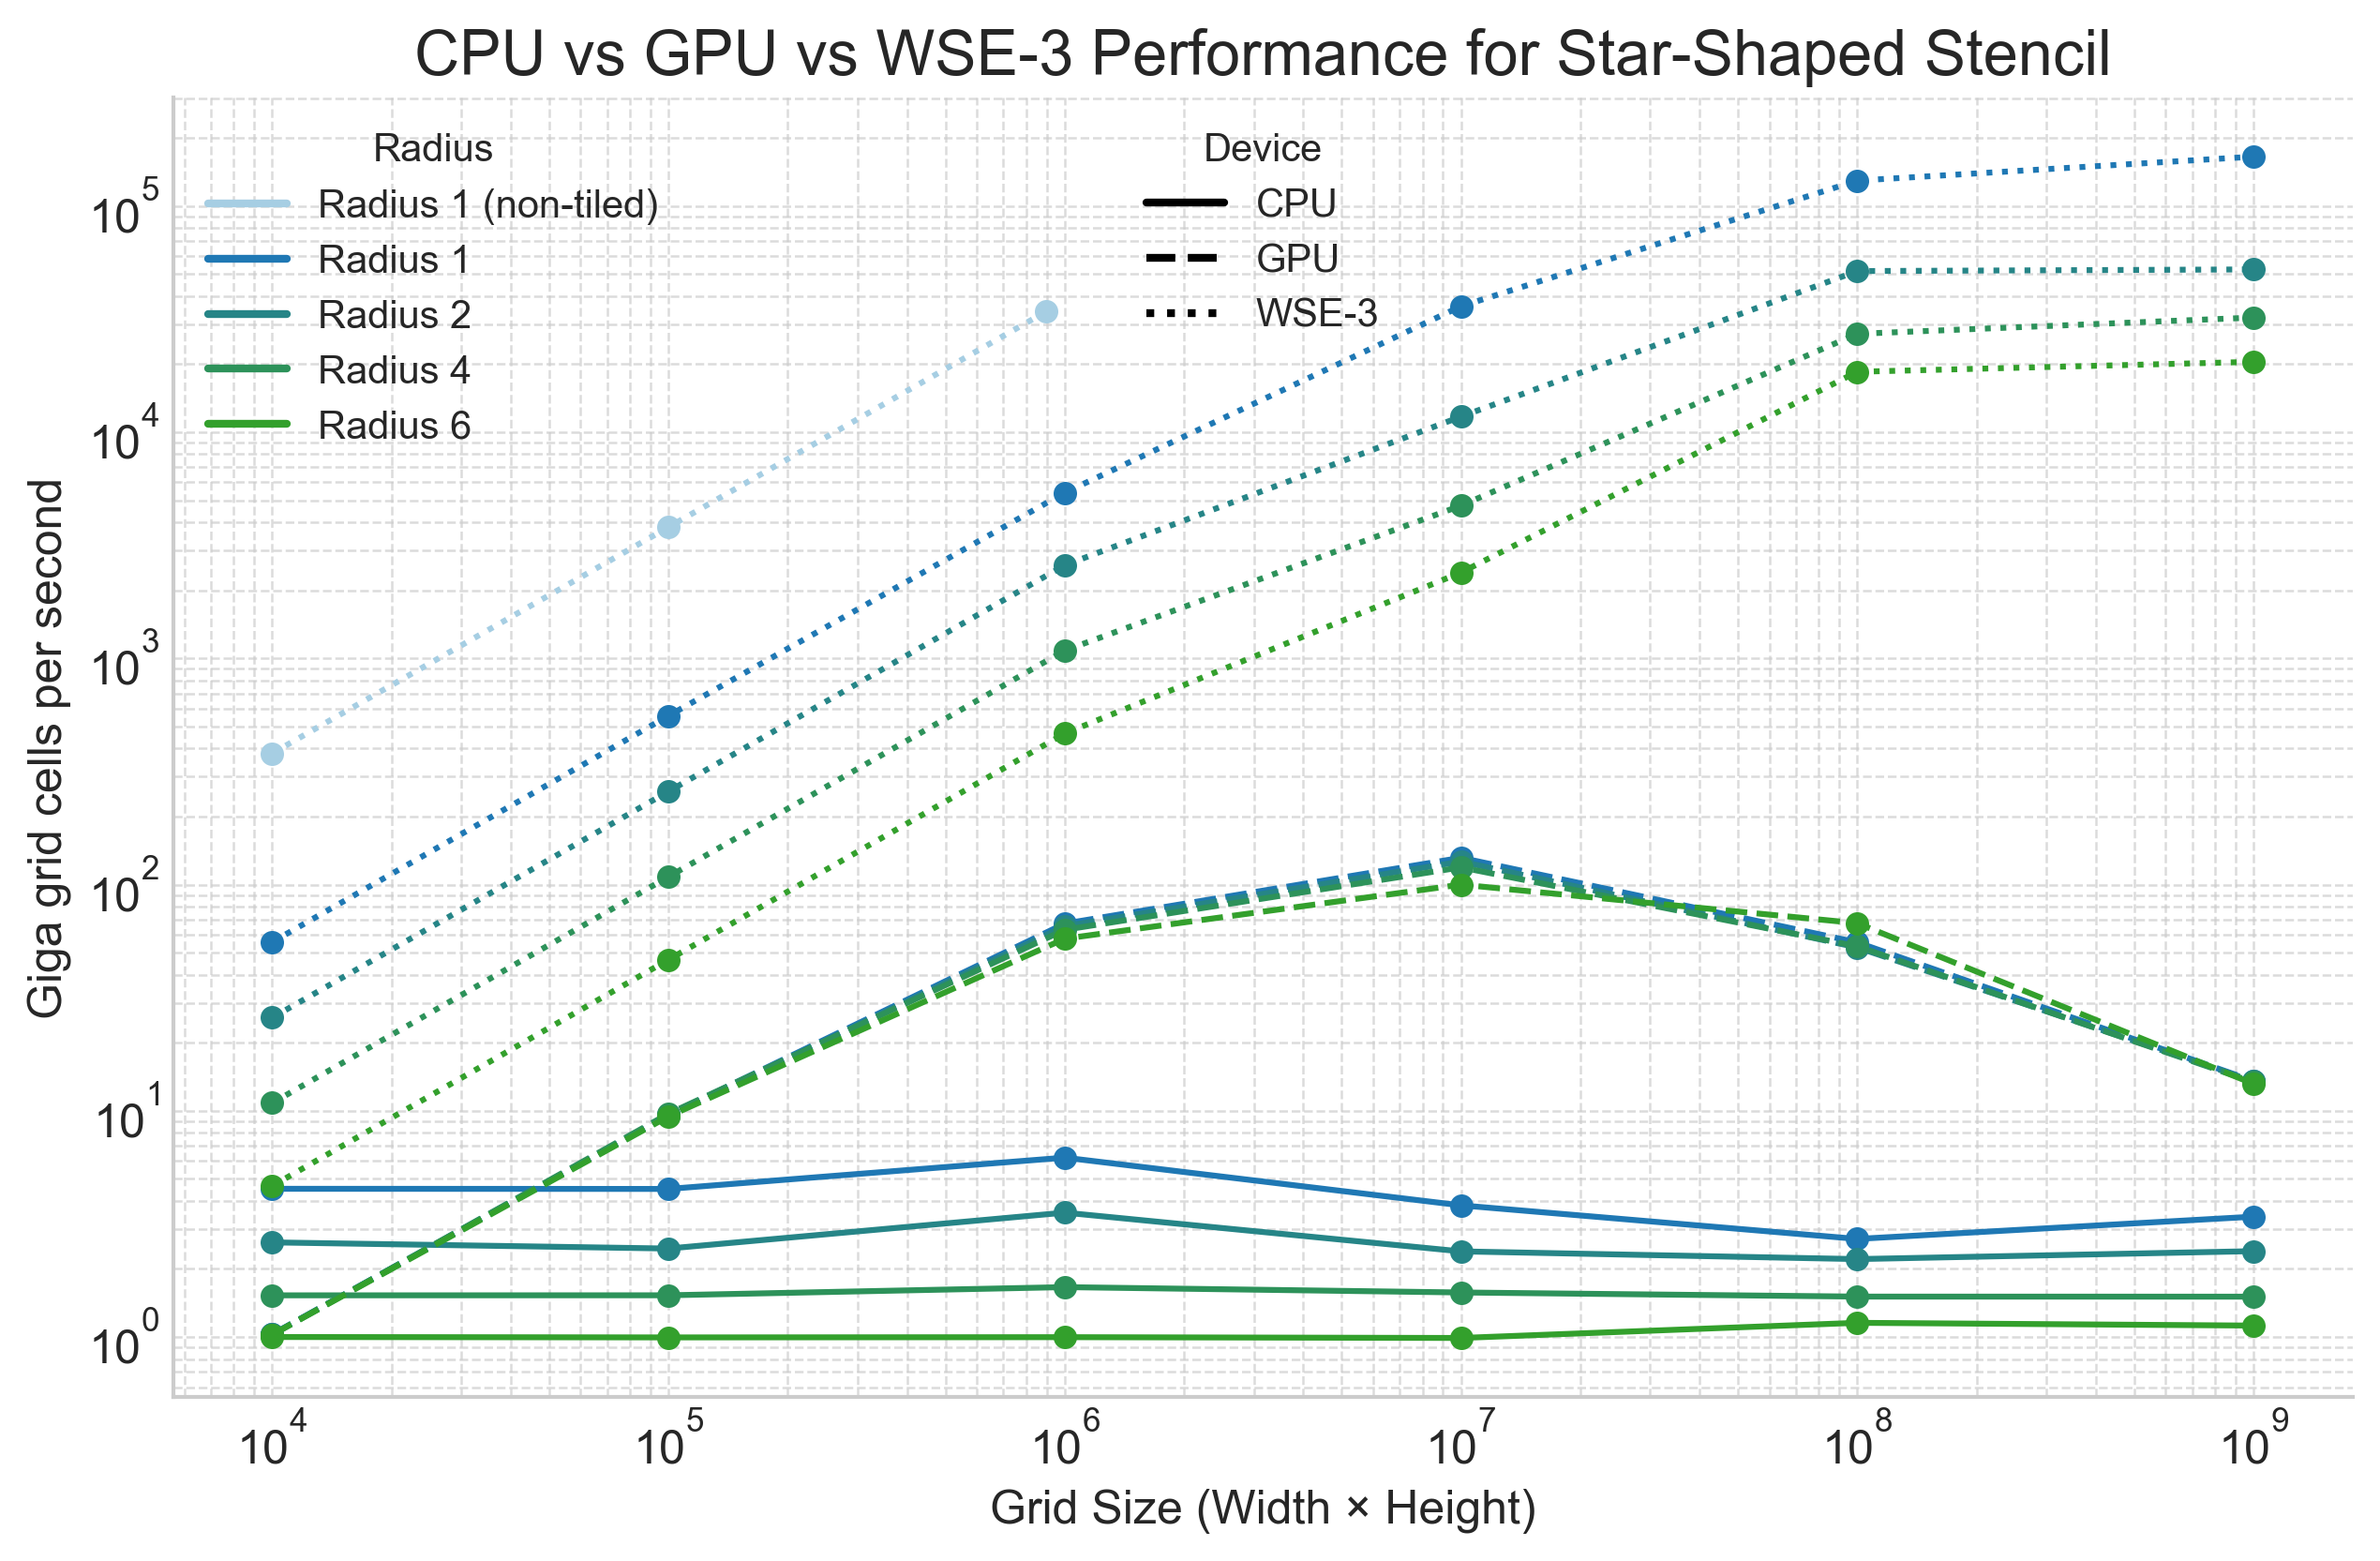
\includegraphics[width=1\linewidth]{gpu_cpu_wse3_constant_product_gcells.png}
    \caption{Comparison of \ac{cpu}, \ac{gpu}, and \ac{wse}-3 performance in Giga-cells per second (Gcells/s) for different grid sizes and radii}
    \label{fig:gpu_cpu_constant_product}
\end{figure}

\subsubsection{\ac{cpu} Performance}
The results, shown in \autoref{fig:gpu_cpu_constant_product}, demonstrate that the \ac{cpu}'s throughput is unaffected by problem size and differs only by a factor of \num{2.3} between its ideal grid size of \num{1e6} and its least ideal grid size of \num{1e8} using radius one. For the largest tested radius of \num{6}, this effect is even smaller at a factor of \num{1.2}.

If the problem was memory-bound, one would assume the \ac{cpu} to be more efficient for small grid sizes that could fit in the faster caches. So its independence of the problem size suggests that it is compute-limited.
This is confirmed by the fact that the \ac{cpu} throughput scales almost perfectly proportionally to the inverse radius.
At a grid size of \num{1e6}, the throughput for the $r=1$ stencil is \num{6.2} times higher than for the $r=6$ stencil, which is \num{6} times as computationally expensive. This proves the system's vast cache and the optimization techniques applied by Devito very effective, shifting the problem from typically being memory-bound to being compute-bound. 

\subsubsection{\ac{gpu} Performance}
Contrary to the \ac{cpu}, we observe that the \ac{gpu} performance differs significantly depending on the grid size, with a peak throughput of \qty{131.4}{Gcells/s} for the optimal grid size of \num{1e7} and a 128x lower throughput for the smallest tested grid size of \num{1e4}. Interestingly, a very large grid size of \num{1e9} also results in a 9.7x lower throughput than the optimal grid size. While looking for a possible explanation for the pronounced optimum at a grid size of \num{1e7}, we find that the required memory of $\num{1e7} \times \qty{4}{\byte} = \qty{40}{\mega\byte}$ fits perfectly into the \qty{50}{\mega\byte} L2 cache of the H100.
Unlike the \ac{cpu}, the \ac{gpu} is unaffected by the radius. So much so that all differences in performance for different radii are more likely to be attributed to measurement errors than to a real difference in the runtime. This strongly suggests that the \ac{gpu} is memory-limited for all different tested grid sizes.

\subsubsection{\ac{wse}-3 Performance}
The \ac{wse}-3 throughput depends on both the grid size and the radius. Its dependence on the radius is significant across all grid sizes with a factor of \num{5.5} between radius \num{2} and \num{6} for a grid of \num{1e4} and a factor of \num{2.6} between radius \num{2} and \num{6} for a grid of \num{1e9} (radius one is not comparable since it uses the computationally less intensive r1-optimized implementation).
The more than linear scaling for small grid sizes can be explained by the fact that these problems use a tile size of \numproduct{1 x 1} for radius \num{1} and \numproduct{6 x 6} for radius \num{6} (because of the radius constraint in \autoref{eq:radius_constraint}), which results in an effective number of \acp{flop} per \ac{pe} of $r^2(8r+1)$.

Further analyzing the \ac{wse}-3's performance, we find that the throughput increases linearly with the grid size for grids of \numrange{1e4}{1e6} elements. This is due to the fact that not all available \acp{pe} can be used for small grids like this and the assumption of perfect weak scaling. When using grid sizes from \num{1e6} to \num{1e8}, the implementation can utilize the whole \ac{wse} and the throughput scales as discussed in \autoref{sec:perf_model_validation}.

The \ac{wse}-3 implementation outperforms the \ac{cpu} and \ac{gpu} for all tested grid sizes and radii with the most significant increase in throughput for the largest grid size of \num{1e9} and radius \num{1} with a factor of \num{12000} compared to the \ac{gpu} and \num{48000} compared to the \ac{cpu}. For these parameters, our implementation reaches a throughput of \qty{165}{\tera cells/s}. Because the throughput for the stencil is independent of the radius on the \ac{gpu}, but not on the \ac{wse}-3, the performance increase from \ac{wse}-3 to \ac{gpu} for the same grid size and radius \num{6} is significantly smaller at \num{1500}.

\section{Achieved Computational Efficiency}
We already discussed how close the throughput of our implementation is to the throughput of the performance model.
Nonetheless, how close an algorithm is to specific hardware peak performance is also an important metric as it is typically used to evaluate the performance of algorithms on different kinds of hardware.

The achieved computational efficiency can be calculated from the cycle counts measured in the earlier experiments, the total number of \acp{flop} executed in these experiments, and the maximum number of \acp{flop} that can be executed per cycle and \ac{pe} on the \ac{wse}.

As described in \autoref{sec:implementation}, the single-cell implementation and the r1-optimized implementation perform \num{6} \acp{flop} per cell, iteration, and \ac{pe}, while the general tiled implementation performs $8r+1$ \acp{flop} per cell, iteration, and \ac{pe}. From the tile sizes used in the different experiments, we first calculate the total number of \acp{flop} ($F_{total}$) per iteration and \ac{pe} as:
\begin{equation}
    F_{total} = t_w t_h (8r+1)
\end{equation}
and then divide by the measured cycle count $C_{measured}$ per iteration to get the average number of \acp{flop} per cycle and \ac{pe} ($F_{avg}$) as:
\begin{equation}
    F_{avg} = \frac{F_{total}}{C_{measured}}
\end{equation}

We find that the maximum number of theoretically possible FP32 operations per cycle and \ac{pe} ($F_{max}$) can be obtained with \texttt{@fadds} instructions, which support a \ac{simd} width of 2 on the \ac{wse}-2 and 4 on the \ac{wse}-3 (\texttt{@fmacs} is not supported in \ac{simd} mode). Using the calculated average number of \acp{flop} per cycle and \ac{pe} $F_{avg}$ and the maximum number of \acp{flop} per cycle and \ac{pe} $F_{max}$, we calculate the theoretically possible percentage of the peak performance $E_{avg}$ as:
\begin{equation}
    E_{avg} = \frac{F_{avg}}{F_{max}}
\end{equation}

\begin{figure}[h]
    \centering
    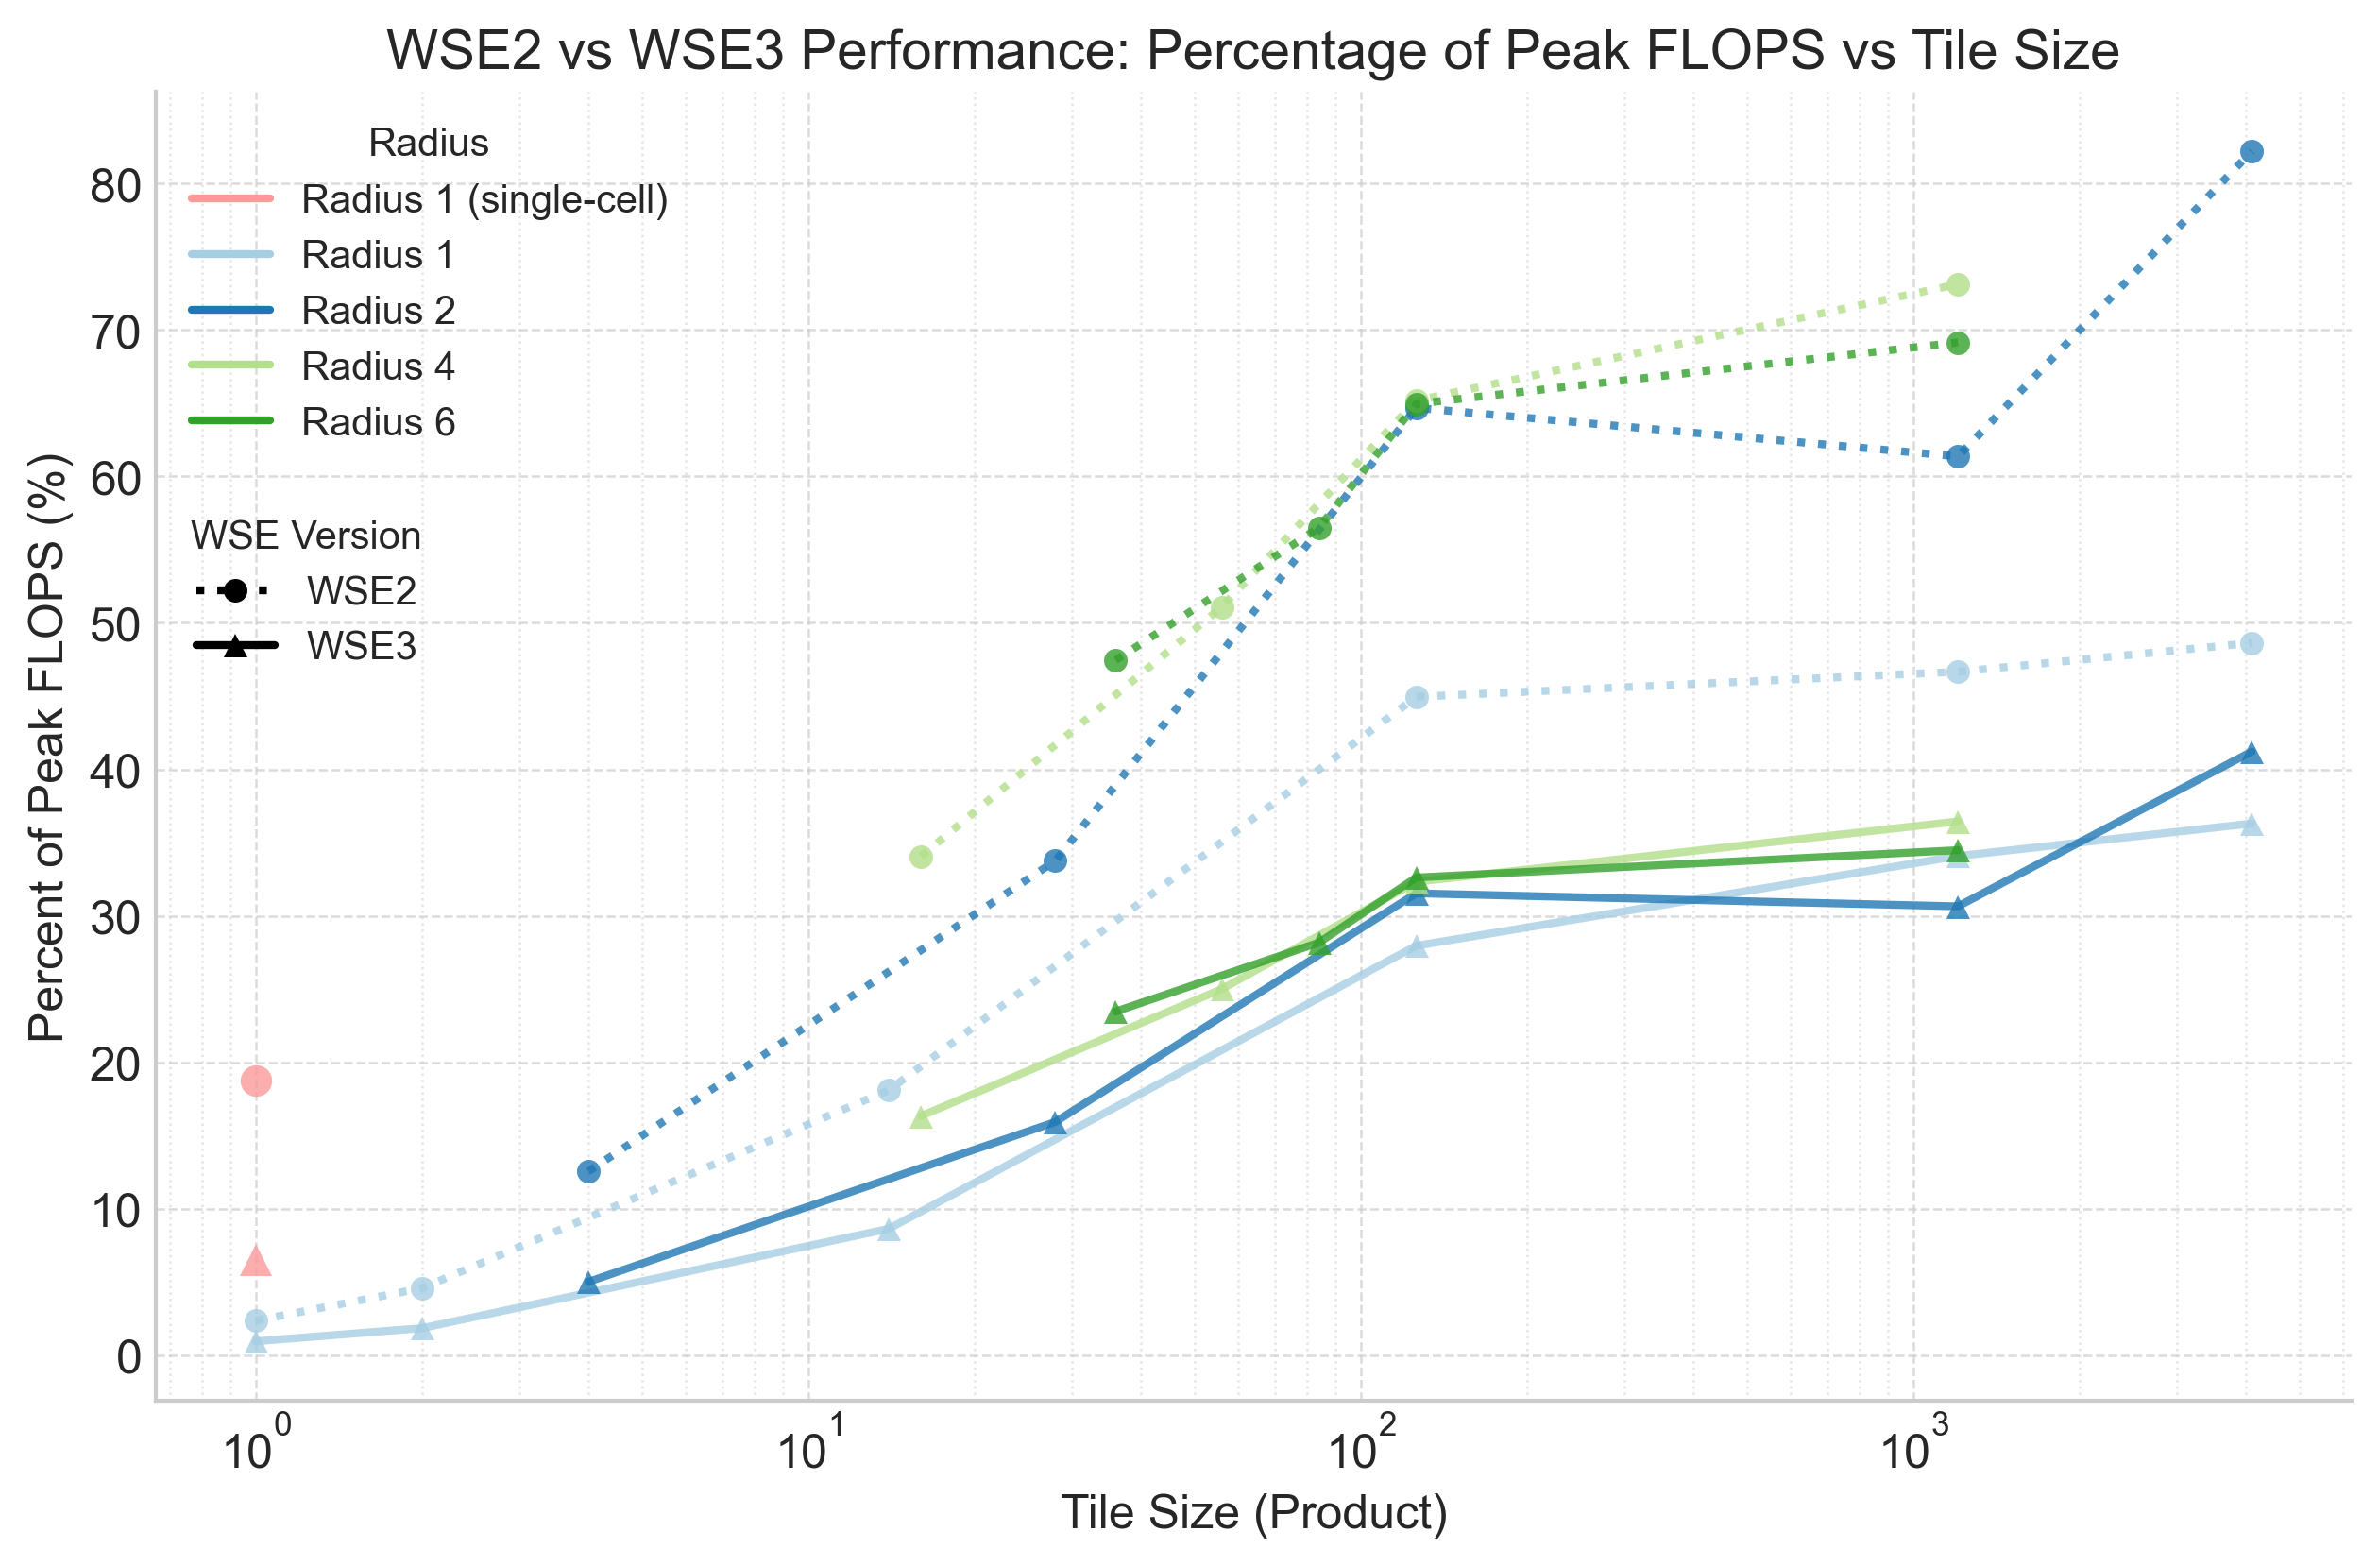
\includegraphics[width=0.7\linewidth]{percent_pflops.png}
    \caption{Extrapolated percentage of peak performance for different tile sizes and radii for \ac{wse}-2 and \ac{wse}-3}
    \label{fig:percent_pflops}
\end{figure}

For radius 2 and the maximum tile size of \numproduct{64 x 64}, we reach \num{82}\% of the peak performance for the \ac{wse}-2 and \num{41}\% for the \ac{wse}-3.
These numbers are extrapolated from our small-scale simulator experiments and assume perfect weak scaling across the entire \ac{wse} as already discussed. 
In general, the achieved percentage of peak performance mostly increases with the tile size. There is no clear trend for the radius, except for radius 1, which is using the r1-optimized implementation and, as discussed in \autoref{sec:theory_performance}, is farthest from the peak performance.

In the optimal configuration, our implementation may reasonably be expected to reach a sustained performance of 1.01 P\ac{flops} for the \ac{wse}-2 and 1.29 P\ac{flops} for the \ac{wse}-3.

\section{Conclusions}
In this work, we demonstrated an efficient implementation for 2D star-shaped stencils targeting the \ac{wse}-2 and \ac{wse}-3 that uses tiling of the problem domain as the core mechanism to increase computation workload relative to communication. We developed a simplified performance model which we used to analyze the scaling properties of the kernel. Furthermore, we validated the performance model with experiments on the cycle-accurate simulator for the \ac{wse}.

In a direct comparison with an NVIDIA H100 \ac{gpu}, our implementation in the simulator for the \ac{wse}-3 reached up to 12000x higher throughput, and when targeting the \ac{wse}-2, a predicted value of 82\% of theoretical FP32 peak performance. Our results prove the effectiveness of tiling and the \ac{wse}'s potential for 2D stencil problems.